\documentclass[journal]{IEEEtran}
\newif\ifblindreview
\ifdefined\BLINDREVIEW\blindreviewtrue\fi
\raggedbottom
% ---------------------------------------------------------------------------
% Paper 4 (dcdtuni docs/manuscripts/paper2) -- IEEE journal draft
% Working title: Differentiable Design Languages
% Status: TNNLS draft 2026-09-15; every number traces to ddl/docs/RESULTS_index.md
% ---------------------------------------------------------------------------
\usepackage[utf8]{inputenc}
\usepackage[T1]{fontenc}
\usepackage{amsmath,amssymb,amsfonts}
\usepackage{bm}
\usepackage{graphicx}
\usepackage{booktabs}
\usepackage{multirow}
\usepackage{algorithmic}
\usepackage{algorithm}
\usepackage{xcolor}
\usepackage{url}
\usepackage[hidelinks]{hyperref}
\usepackage[capitalise]{cleveref}
\usepackage{placeins}
% TNNLS readers meet a figure where the text first cites it: relax IEEEtran's float
% deferment, and \FloatBarrier before every \section pins each float to its section.
\setcounter{topnumber}{4}
\setcounter{dbltopnumber}{2}
\renewcommand{\topfraction}{0.92}
\renewcommand{\dbltopfraction}{0.92}
\renewcommand{\textfraction}{0.08}
\renewcommand{\floatpagefraction}{0.85}
\renewcommand{\dblfloatpagefraction}{0.85}

\newcommand{\platform}{\ifblindreview a production data-centre digital-twin platform\else the DCTwin platform\fi}
\newcommand{\todo}[1]{\textcolor{red}{[TODO: #1]}}
\newcommand{\ph}[1]{\textcolor{blue}{#1}}           % placeholder numbers
\newcommand{\ddl}{DDL}
\newcommand{\Jobj}{J}
\newcommand{\design}{\bm{d}}
\newcommand{\soft}{\tilde{\bm{p}}}
\newcommand{\task}{\tau}
\newcommand{\E}{\mathbb{E}}
\newcommand{\Var}{\mathrm{Var}}
\DeclareMathOperator*{\argmin}{arg\,min}

\begin{document}

\title{Differentiable Design Languages: Post-Training Language-Model Design Agents with Adjoint Gradients from Physics Simulators}

\ifblindreview
\author{Anonymous Authors}
\else
\author{Tianyu~Li,
        Qingang~Zhang,
        Hoanghuy~Nguyen,
        Zhiwei~Cao,
        Ruihang~Wang,
        Binyang~Song,
        and~Yonggang~Wen,~\IEEEmembership{Fellow,~IEEE}%
\thanks{This work was supported in part by the Ministry of Education, Singapore,
under its Academic Research Fund Tier 1 of RG104/23, in part by A*STAR under its
MTC Programmatic of M23L9b0052, and in part by Leoch Battery Pte. Ltd.
A conference version of parts of this work appeared at the AIFLUIDS 2026
conference~\cite{li2026dctwin}.  \emph{(Corresponding author: Yonggang Wen.)}}%
\thanks{T. Li is with the AI-X Programme, Interdisciplinary Graduate Programme, and the College of Computing and Data Science, Nanyang Technological University, Singapore 639798.  Q. Zhang, H. Nguyen, Z. Cao, and Y. Wen are with the College of Computing and Data Science, Nanyang Technological University, Singapore.  R. Wang is with the School of Information Science and Engineering, Yunnan University, Kunming, China.  B. Song is with the School of Mechanical and Aerospace Engineering, Nanyang Technological University, Singapore.}%

}
\fi

\ifblindreview
\markboth{IEEE Transactions on Neural Networks and Learning Systems}{Anonymous submission}
\else
\markboth{IEEE Transactions on Neural Networks and Learning Systems}{Li \MakeLowercase{\textit{et al.}}: Differentiable Design Languages}
\fi

\maketitle

% ===========================================================================
\begin{abstract}
Engineering design agents emit discrete decisions, so a differentiable solver's
adjoint reaches them only as a scalar reward.  We introduce differentiable
design languages: typed design-action vocabularies whose token-level relaxations
are soft designs an instrumented production solver simulates, and whose one-hot
limit recovers the hard design up to a measured closure floor.  On a production
liquid-cooling solver the relaxation leaves the sparsity pattern and Newton path
unchanged, so the implicit-function-theorem adjoint reuses an assembled Schur
complement.  It matches central differences to the finite-difference floor:
$3\times10^{-10}$ at interior points, $1.4\times10^{-3}$ at one-hot closed-branch
coordinates.  % source: E0b 20260916T012509Z
Post-training a 4-billion-parameter model with this gradient converts infeasible
designs into feasible ones, but spends design quality to buy constraint
satisfaction.  Adjoint fidelity is decision-type dependent (Spearman $0.94$ on
catalogue edits, $0.31$ on structural re-assignments).  % source: E1b 20260915T150205Z_race5seed_calibbugfix, E1d_edit_ranking 20260915T150207Z_edit5seed
A discrete edit-selection protocol replaces cosine fidelity as the decision
criterion.  On it the exact adjoint out-ranks the scalar-reward arm over ten
policy points (one-sided exact signed-rank $p=0.0020$).  % source: E1d 20260915T150207Z_edit5seed
At matched budget on the $6{,}599$-parameter factorised policy the pathwise gradient halves scalar-reward regret over five
seeds and five tasks (paired exact $p=6.0\times10^{-8}$).  Yet on the production
solver the same gradient regresses against its own warm start in the pooled
per-(seed, task) rows at five seeds, where the seed-mean primary stays inseparable.  % source: v2B 20260916T033403Z; amortisation Sec. VII-E
\end{abstract}

\begin{IEEEkeywords}
Adjoint methods, differentiable physics, engineering design automation, large
language model agents, post-training.
\end{IEEEkeywords}

% ===========================================================================
\FloatBarrier
\section{Introduction}
\label{sec:intro}

\IEEEPARstart{E}{ngineering} design problems are mixed: a designer chooses a
\emph{structure}---a topology, an assignment, a catalog part---and then tunes
the \emph{continuous} parameters that the structure exposes.\ifblindreview\footnote{A conference version of parts of this work exists under the blinded citation~\cite{li2026dctwin}.}\fi  The second half
of this problem has been transformed by differentiable simulation.  Adjoint
methods deliver the gradient of an objective with respect to every continuous
parameter at the cost of one extra linear solve~\cite{giles2000adjoint}, and
differentiable solvers make that gradient available to any downstream
learner~\cite{hu2020difftaichi}.  The first half has,
more recently, been handed to large language models (LLMs): agents that read
specifications, catalogs and constraints and emit candidate structures as
text or code~\cite{ma2024sga,jadhav2026mechdesigner,phythesis2025}.  The prevailing pattern is by now standard: the LLM proposes discrete
structure, the differentiable solver optimises continuous parameters, and the
outcome returns to the LLM as a number in its prompt.

This pattern wastes most of what the simulator knows.  Once a structure is simulated, the adjoint yields the sensitivity of the objective to
every parameter of that structure.  Because the agent's proposal is a sequence of
discrete tokens, none of this sensitivity can be back-propagated into the agent.  The agent therefore learns, if it learns at all, from a scalar reward.
Simulator-feedback post-training methods such as reinforcement learning from
simulator feedback (RLSF)~\cite{scidesignbench2026} or
GRPO~\cite{shao2024grpo} must estimate the gradient of expected reward with
score-function (REINFORCE) estimators
\cite{williams1992reinforce,mohamed2020mcgrad}.  These estimators are
unbiased but their variance grows with the size of the action space, and each
sample costs one physics simulation.  When a simulation takes minutes, the
variance of the credit-assignment signal---not the capacity of the model---is
what limits how much design knowledge can be amortised into the agent's
weights.

Two lines of recent work suggest that the gradient path can be closed.  In
the LLM-alignment literature, GRADE~\cite{grade2026} and DiffRO~\cite{diffro2025}
replace policy gradients with direct back-propagation through a
Gumbel-softmax straight-through relaxation of token sampling~\cite{jang2017gumbel,maddison2017concrete,bengio2013ste}.  They report an order-of-magnitude lower gradient variance than REINFORCE when
the reward is differentiable in the tokens.  In the physics literature,
physics-driven generators~\cite{jiang2019glonet} and differentiable-physics
control platforms back-propagate adjoint
gradients into the parameters of neural designers and controllers whose
outputs are continuous.  Neither line addresses the case in which the
designer emits \emph{discrete structural decisions} and the reward is a
\emph{physics solver}: the relaxed token distribution must first be turned
into something the solver can simulate.

\Cref{fig:pipeline} closes the loop this paper studies: the agent's tokens relax
into a soft design the instrumented solver simulates, and the adjoint of that solve
returns through the relaxation to the token logits.

\begin{figure*}[!t]\centering
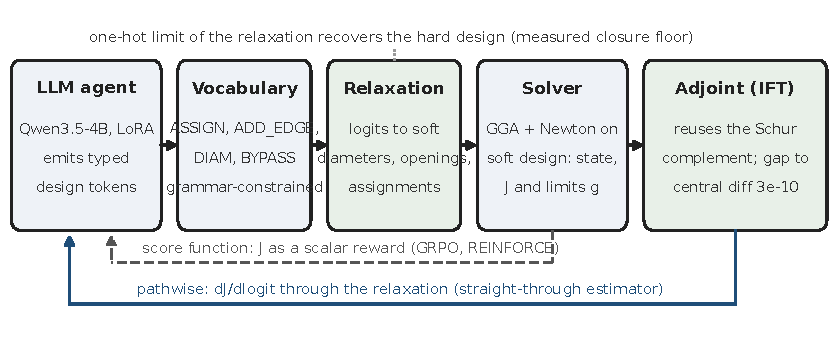
\includegraphics[width=\linewidth]{figures/fig_pipeline.pdf}
\caption{The differentiable-design-language loop.  A language-model agent emits
typed design actions, and a relaxation map turns the token distributions into soft
physical parameters that the instrumented production solver simulates.  The
implicit-function-theorem adjoint of that solve returns through the relaxation to
a gradient on the token logits (solid path), against a score-function route that
sees only the scalar objective (dashed path).  The one-hot limit of the relaxation
recovers the hard design up to the measured closure floor.}
\label{fig:pipeline}\end{figure*}

\subsection{This paper}

We introduce \emph{differentiable design languages} (\ddl{}): a typed vocabulary
of design actions---both benchmarks instantiate \texttt{ASSIGN} and
\texttt{DIAM}, while \texttt{ADD\_EDGE} and \texttt{BYPASS} remain vocabulary slots
whose relaxation is open work.  It comes with a \emph{relaxation map} $\rho$ that
sends the categorical distribution over each design token to a soft physical
parameter.  The map has two properties: \emph{consistency}, a one-hot
distribution recovers the hard design, and \emph{physical closure}, any
probability vector yields a system the solver can
simulate.\footnote{Closure is a design property of the relaxation map, not an
empirical guarantee of a particular Newton implementation.  \Cref{sec:e0lc}
reports the closure sweep and its exception rate.  At the deployed
configuration every one of the $90$ relaxed solves converges, and $5$ of $90$
one-hot compiles are rejected by the topology check (a single dead-end design). With damping disabled a non-converging oscillation of the undamped Newton step
appears, which the deployed damped solver never exhibits.  Any claim of the form
``every probability vector is simulable'' should therefore be read as holding
for all but a measured small fraction.}.  A soft rack-to-unit assignment, for
example, becomes a convex combination of hydraulic conductances bounded away
from singularity.  Closure is what ordinary text decoding lacks, and it makes
the chain $\theta\!\to\!\text{logits}\!\to\!\text{tokens}\!\to\!\soft\!\to\!\Jobj$
differentiable end to end.  The adjoint gradient $\partial\Jobj/\partial\soft$
then flows through a Gumbel-softmax straight-through estimator into the LLM
parameters $\theta$, at one forward and one adjoint solve per sample
(\ref{eq:pathwise}).
% source: ddl/case/benchB/E0f_closure_repair/loggers/20260915T201056Z_gpuserver/
%         (closure sweep: 90 relaxed solves, 5 of 90 dead-end at C_min=1e-5).

We do not claim that this \emph{pathwise} estimator is unbiased---it is not---nor
a framework result about pathwise versus score-function estimators.  Low
variance and high bias near nonsmooth events, bias corrections and unbiased
mixtures are all established
\cite{suh2022diffsim,onoda2026ddcg,scheffler2026cfobg,hpo2026}.  Nor is the
interesting question \emph{whether} physics gradients can be routed into a
language model: once a \ddl{} exists they can, and every language-model run in this paper uses
it at 4B (\cref{sec:e2}).  The questions this paper answers are three, all about measurement.  \emph{First}, can a relaxation for genuinely
\emph{structural} discrete decisions be made physically closed inside a
production solver, and is the resulting adjoint exact?  The nonsmoothness prior
work corrects for lives in the dynamics; ours lives in the model's output, which
makes it a modelling object rather than an estimator correction.
\emph{Second}, what is that adjoint worth, and does the answer depend on the
\emph{type} of decision?  It does: catalogue edits rank at $0.94$ while
structural re-assignments rank at $0.31$ on the production solver, and we quote
no ratio of the two gaps because its denominator carries no interval.
\emph{Third}, how should an estimator be scored when the artefact that ships is
a hard design?  Cosine against a high-sample unbiased reference turns out to be
informative about the relaxed objective and uninformative about the deployed
one, and we replace it.

A fourth question bounds the first three: the objective defining our regret is
itself a search, and gradient-free local search solves a task in two seconds, so
% source: two seconds = the 400-evaluation cap of the gradient-free search arm at
%         7 ms per hard compile at N=10 (ddl/case/analysis/solve_scaling/loggers/
%         20260916T1420Z_gpuserver/results_solve_scaling.json); the median 186
%         evaluations of ddl/case/policy/greedy_and_oracle is 1.3 s at the same rate.
what does post-training buy at all?  We answer with a break-even analysis on two axes.  A $6{,}599$-parameter
non-language policy is post-trained with the same gradient under its own step
budget (Supplementary Sec.~S-II). A prompt-level sensitivity baseline hands
the same neighbourhood information to the model as text instead of as a gradient.  The
answers are not flattering to the language model, and we report them as
measured.

We study these questions on two physical environments.  The first is a
purpose-built, enumerable differentiable thermo-hydraulic network benchmark in
which every single-step structural edit can be evaluated exactly against a
ground-truth gradient of the expected objective.  The second is the
liquid-cooled data-center pipe network of \platform
platform~\cite{li2026dctwin}, whose compiler turns \ddl{} actions into
schema-validated cooling-network descriptions and whose Newton-based hydraulic
solver provides the adjoint.  Data-center liquid cooling is a fitting test case:
the structural decisions are genuinely discrete, and the continuous
re-optimisation of flows and pump speeds can mask or expose their
value~\cite{jadhav2026codesign}.  The design task also recurs across facilities,
which is what makes amortising design knowledge into a model worthwhile.

% ===========================================================================
% sections_v2/contributions.tex -- round-8 rewrite: a qualitative list only.
% Every number in this paper lives in Sec. VII and in the % source: comments
% there.  This file states what the paper contributes and what it does not
% claim, with section pointers and no quantitative claim of its own, so that
% the introduction can never drift from the results again.
% Cross-file labels: sec:rw-concurrent is defined in sections_v2/related_work.tex.
% ===========================================================================
\subsection{Contributions}
\label{sec:contributions}

\begin{enumerate}

\item \textbf{A physically closed relaxation for discrete structural decisions
  inside a production water-network solver, with an adjoint that matches central
  differences to the finite-difference floor ($3\times10^{-10}$ at interior points,
  $1.4\times10^{-3}$ at one-hot closed-branch coordinates)}
  (\cref{sec:method,sec:e0lc}).  The relaxation lives inside the solver's own
  friction law, so every probability vector over design tokens is a network the
  unmodified solver can simulate.  Closure is a measured neighbourhood property:
  the floor below which unchosen branches vanish is swept, and its price
  reported at every value.

\item \textbf{The bias of a first-order pathwise gradient depends on the
  \emph{type} of decision it is asked about} (\cref{sec:e0lc,sec:e1lc}).  On
  the production solver the same adjoint ranks catalogue edits faithfully and
  structural re-assignments poorly, and no estimator in the compared family
  repairs the asymmetry.

\item \textbf{A measurement protocol for post-training design agents, and the
  accounting it produces} (\cref{sec:e2,sec:e2B} and Supplementary Sec.~S-VII).  Paired per-task
  tests at the stated seed count, an endpoint-versus-best-checkpoint census over
  every archived run, and a decomposition of each objective reduction into
  design and penalty parts.  Applied here it shows post-training buying
  constraint satisfaction by spending design quality on one benchmark, and
  regressing against its own warm start on the other.  The protocol's one
  unqualified positive is at matched budget on a 6{,}599-parameter factorised
  policy, where pathwise halves scalar-reward regret (\cref{sec:baselines}).
  % source: ddl/case/analysis/v2A_table/loggers/20260915T175120Z_gpuserver/
  %         results_v2A_table.json -> table, paired_wilcoxon; break-even from
  %         ddl/case/analysis/consistency_inputs/loggers/20260915T154717Z_gpuserver/
  %         results_consistency.json -> c_breakeven.
  The break-even arithmetic of \cref{sec:discussion} states the amortisation
  threshold as a falsifiable prediction for the minutes-per-solve regime.

\item \textbf{A protocol for scoring gradient estimators when the artefact
  that ships is a hard design} (\cref{sec:e1lc,sec:discussion}).  The
  conventional metric, cosine against a high-sample unbiased reference, is only
  a description of a nine-arm table here (\cref{sec:e1lc}), so we do not use it.
  The substitute is discrete edit selection, validated by a deterministic probe:
  paired over ten confident policy points the exact adjoint beats the
  scalar-reward arm (\cref{sec:e1lc}, one-sided $p=0.0020$).
  % source: ddl/case/analysis/round10_reanalysis/loggers/20260915T201839Z_gpuserver/
  %         results_round10.json (rho, permutation p); edit-selection paired test from
  %         ddl/case/benchB/E1d_edit_ranking/loggers/20260915T150207Z_edit5seed.

\item \textbf{Benchmark validity as a result} (\cref{sec:setup} and
  Supplementary Sec.~S-X).  The first benchmark of this line of work failed a
  physicality audit that its own labels made computable.  The repair is verified
  against enumeration wherever enumeration is possible, and every result carries
  the physics configuration it was run under.

\end{enumerate}

\subsection{What we do not claim}
\label{sec:notclaim}

Four negative statements bound the five positive ones.  We do not claim that
pathwise estimators beat score-function estimators in general; our evidence is
about decision types, not estimators.  We do not claim that post-training
improves design quality: on both benchmarks it either buys feasibility at a
design cost or regresses against its warm start.  We do not claim a scale
result, since no 27B run is reported here
(\cref{sec:e27b}), nor that a language model beats constrained search where
search is cheap (\cref{sec:baselines}).  A concurrent paper made the Global
Gradient Method differentiable before this draft froze \cite{mu2026gga}; our
relaxation and the weight-level use of its adjoint are independent of that work
(\cref{sec:rw-concurrent}).


% ===========================================================================
\section{Related Work}
\label{sec:related}

When a model emits discrete symbols and the objective depends on them, the
gradient of the expected objective is classically estimated with the
score-function estimator \cite{williams1992reinforce,greensmith2004variance,schulman2015gradient}.  Its group-normalised
form, GRPO, is now the default for post-training language models
\cite{shao2024grpo}.  Such estimators are unbiased but their variance grows
with the number of sampled symbols, and here every sample costs one physics
simulation \cite{mohamed2020mcgrad}.  The alternative relaxes the sampling step:
Gumbel-softmax / Concrete combined with a straight-through estimator makes the
sampled symbol a differentiable function of the logits, at the price of bias
\cite{jang2017gumbel,maddison2017concrete,bengio2013ste,kingma2014auto,tucker2017rebar,grathwohl2018backpropagation}.  That construction has
reached LLM post-training as direct back-propagation through token sampling
\cite{grade2026,diffro2025,hu2023abs}.  In the physics-simulation literature the
same bias--variance account is worked out in detail \cite{suh2022diffsim}.
Variance control rather than bias removal dominates in practical deployments
\cite{onoda2026ddcg}, a corrected first-order formula restores unbiasedness at
discontinuities \cite{scheffler2026cfobg}, and a mixed
estimator preserves unbiasedness for hybrid discrete--continuous actions
\cite{hpo2026}.  This paper contributes no estimator, no bias bound and no
unbiasedness result; all three exist in the work just cited.

What is missing there is the object the estimators act on.  In the
physics-estimator line the non-smoothness is a property of the \emph{dynamics}---contact, a status switch, stiffness---while the design or action space is already
continuous.  In the token-relaxation line the discrete object is a text token, whose
relaxation needs no physical interpretation.  Our
setting inverts this: the non-smoothness is in the \emph{design} the language
model emits, and the relaxed object must first be a system a production solver
can simulate at all.  That requirement---physical closure of the relaxation---is
a modelling object, not an estimator correction, and it is the whole of our
first contribution (\cref{sec:contributions}).

\subsection{Physics gradients into learned designers}
\label{sec:rw-designers}
A parallel line feeds gradients from differentiable simulators into the weights
of neural designers, from metasurface generators to differentiable-programming
systems \cite{jiang2019glonet,hu2020difftaichi,um2020solver,holl2020learning}. It includes end-to-end design on
top of \emph{learned} simulators \cite{allen2022physicaldesign,raissi2019pinn} and
standalone differentiable flow-control benchmarks \cite{fluidgym2026}.  In
topology optimisation the designer's
output is a density field, so the gradient path is closed by construction,
whether by SIMP or by a meta-learned neural field
\cite{bendsoe1989simp}.  The most instructive recent case
conditions a Bernoulli flow-matching generator on the adjoint sensitivity field,
argued via the data-processing inequality to be the information-theoretically
optimal conditioning signal \cite{topotransformer2026}.  There the adjoint
enters as an \emph{input field} to a trained generator; here it enters as a
\emph{gradient with respect to the designer's weights} from a single simulation
of the design the model itself proposed.  Mechanically our adjoint is an
ordinary implicit-function-theorem derivative of a fixed-point solver, and we
claim no part of that construction as new
\cite{giles2000adjoint,lorraine2020implicit,knoll2004jfnk}.  The gap we address
is where that construction fails. When the designer emits a sequence of
categorical structural decisions there is no continuous field to differentiate,
and the relaxation must be supplied by the design language.

\subsection{Language-model agents for physical design}
\label{sec:rw-llm}
LLM agents propose structures, write simulation code and iterate on numerical
feedback, alternating discrete hypotheses with differentiable refinement or
solver-in-the-loop iteration
\cite{ma2024sga,jadhav2026mechdesigner,li2026dctwin,chang2023chipnemo,boiko2023autonomous}.
Prior work couples an LLM layout generator to a gradient-free
evolutionary level \cite{phythesis2025}.  A newer line post-trains language
models on simulator feedback.  SciDesignBench reports that the best zero-shot
model reaches $29.0$\% success on 520 inverse-design tasks, and that a
simulator-feedback recipe raises single-turn success by $8$--$17$ points
\cite{scidesignbench2026}.  LEAPBench finds that scoring trajectories rather
than final outcomes changes the best-model decision on $53$\% of tasks, and
that LLMs do not outperform a classical Bayesian baseline
\cite{zhang2026leap}.  In all of these the simulator's influence is mediated by
a scalar or by text: either the numbers re-enter through the prompt and nothing
is amortised into the weights. Or they enter as a reward and credit assignment
falls back on a score-function estimator.  We differ in the interface, not in
the ambition: the simulator's Jacobian, not its output value, reaches the
model's parameters.  We adopt both prescriptions of \cite{zhang2026leap}:
report design quality per physics evaluation, and compare against
gradient-free search rather than against another language model.

\subsection{Discrete structural design with continuous physics}
\label{sec:rw-structural}
The underlying engineering problem has a mature literature outside machine
learning.  Topological derivatives quantify the first-order effect of an
infinitesimal structural perturbation \cite{sokolowski1999topological}.
In the district-heating line the adjoint itself resolves the discrete structure:
projection, penalisation and continuation relax pipe presence and discrete
diameters \cite{blommaert2020adjoint}, and pipe placement is relaxed by a
penalisation benchmarked against an exact MINLP \cite{wack2022energy,wack2023gap}.  Benders-type decomposition separates a discrete
master from a continuous subproblem
\cite{geoffrion1972benders}.  The hydraulic steady state we
differentiate is the Global Gradient Method solved by damped Newton iteration
\cite{todini1988gga,knoll2004jfnk}.  For liquid-cooled data centres, control is
well established under a given topology \cite{lcopt2025}, and design-side
co-design work enumerates integer partitions of coolant distribution units
against a reduced-order surrogate, one instance at a time
\cite{jadhav2026codesign}.  These are the
right answers when the structural space is enumerable; our aim is
complementary, to make the structural decision itself differentiable so that the
physics gradients these methods already compute amortise into a model.
Ground-structure topology optimisation is the classical precedent for a
relaxation whose every relaxed point is a valid structure
\cite{dorn1964automatic,guest2004minimum}.  What we add is a relaxation indexed by
the decoder's categorical distribution over typed tokens, whose Jacobian lands in
logit space.  Its one-hot limit recovers the hard design with the sparsity pattern
and Newton path unchanged.  Neural combinatorial optimisation and grammar-constrained
decoding supply further components we reuse, and neither attaches a simulator
adjoint to the policy's parameters
\cite{vinyals2015pointer,willard2023guided}.
The deep-RL evaluation literature sets the reporting standard we adopt
\cite{agarwal2021precipice,henderson2018matters}.  The optimiser itself combines
LoRA, a clipped surrogate and truncated Gumbel sampling
\cite{hu2021lora,schulman2017ppo,kool2019stochastic}.

\subsection{Concurrent work: an exactly differentiable water-network solver}
\label{sec:rw-concurrent}
Mu et al.\ \cite{mu2026gga} make the Global Gradient Method itself exactly
differentiable: their backward pass reuses the terminal factorisation of the
forward pass, so one extra sparse solve returns every parameter's gradient.
Across 8{,}140 frames of 52 networks the largest head deviation from EPANET~2.2
is $1.137\times10^{-13}$\,ft, and on the 905-pipe L-TOWN benchmark one adjoint
solve replaces 906 simulations.  This is a stronger and more thoroughly
validated version of the adjoint we attach in \cref{sec:benchB}, and we regard
the construction as established: a reader who needs a production-grade
differentiable hydraulic solver should use theirs.  The two works are
complementary in a way that sharpens our claim.  Two of their decisions---roughness calibration and leak localisation---are
continuous, while sensor placement is a discrete $k$-subset selection resolved by
submodular lazy greedy over the adjoint's Fisher information; their backward pass
freezes the combinatorial configuration the forward pass converged to.  That greedy
buys adjoint information without a relaxation; a relaxation adds a gradient path
into a parametric model.  Our problem is exactly the perturbation that would change that
configuration: a rack reassigned to another coolant distribution unit, a branch
added or isolated, a pipe class changed.  Nothing in \cite{mu2026gga} relaxes a
discrete decision; the words \emph{language model}, \emph{Gumbel},
\emph{straight-through} and \emph{token} do not occur in it.

\subsection{Positioning}
\label{sec:rw-positioning}
The positioning table of Supplementary Sec.~S-VIII places the present work
against the groups above; its two new columns are summarised here.  Two
columns are new relative to the usual positioning table.  ``Relaxation is
physical'' asks whether every point of the relaxed design space is a system the
solver can simulate, a property we certify and no estimator paper needs.
``Pathwise bias'' records that the framework-level answers are owned by
\cite{suh2022diffsim,onoda2026ddcg,scheffler2026cfobg,hpo2026} while ours is a
measurement resolved by decision type in one engineering domain.  The
distinguishing combination remains a \emph{discrete} structural design emitted
by a \emph{language model} whose parameters receive a \emph{solver adjoint}
through a relaxation that is itself a physical design.  Each ingredient exists;
the object that connects them does not.



% ===========================================================================
\FloatBarrier
\section{Problem Setting}
\label{sec:problem}

A design task $\task$ specifies loads, sites, a component catalogue and
textual constraints.  A design is a sequence of typed decisions
$\design=(a_1,\dots,a_T)$, $a_t\in\mathcal V_t(\design_{<t})$, produced by a
policy $\pi_\theta(\design\mid\task)$.  In this paper the policy is a language
model with LoRA parameters $\theta$ decoding under a grammar (\cref{sec:method}).
Each design compiles to physical parameters $\bm p(\design)$ of a steady-state model
$R(\bm q;\bm p,\task)=0$ with state $\bm q$ (pressures, flows, temperatures).  An
objective $\Jobj(\design,\task)=\ell(\bm q^*(\bm p),\bm p)$ scores it, combining
operating cost, capital cost and constraint penalties.  Post-training minimises
\begin{multline}
  \mathcal L(\theta)=\E_{\design\sim\pi_\theta(\cdot\mid\task)}\big[\Jobj(\design,\task)\big] \\
  +\beta\,\mathrm{KL}\big(\pi_\theta\,\|\,\pi_{\mathrm{base}}\big)
  +\lambda_r\,\mathcal L_{\mathrm{replay}}(\theta),
  \label{eq:objective}
\end{multline}
where the KL term (on the decision distributions) and the replay term
(cross-entropy on the base model's own answers to unrelated prompts) guard
against forgetting.  Every estimator for the first term pays one physics
evaluation per sampled design; we report design quality reached per physics
evaluation on held-out tasks.

% ===========================================================================
\FloatBarrier
\section{Differentiable Design Languages}
\label{sec:method}

\subsection{Vocabulary and grammar-constrained decoding}
A \ddl{} fixes, for each decision slot $t$, a small candidate set of
\emph{single} vocabulary tokens $\mathcal V_t$ (for example \texttt{A}/\texttt{B}/\texttt{C}
for the CDU of rack $i$, \texttt{1}/\texttt{2}/\texttt{3} for its pipe
class).  The surrounding scaffold text (\texttt{R1: CDU=\_ DN=\_}) is forced by
the decoder, so the model's only degrees of freedom are the decision tokens
and every sampled sequence is a syntactically valid design.  Decoding runs
autoregressively with a KV cache; at slot $t$ the next-token logits are
restricted to $\mathcal V_t$, giving a categorical
$\pi_\theta(a_t\mid\design_{<t},\task)$.  A second, teacher-forced pass over the
completed sequence returns the same restricted logits with gradient
(only the $T$ needed rows of the vocabulary projection are computed).

\subsection{Relaxation map}
Let $y_t\in\Delta^{|\mathcal V_t|}$ be a probability vector over the candidates
of slot $t$.  The relaxation map $\rho$ sends $(y_1,\dots,y_T)$ to soft
physical parameters $\soft$ with two properties.  (i)~\emph{Consistency in the hard limit}: one-hot
inputs give $\rho(\mathrm{onehot}(\design))=\bm p(\design)$ as $C_{\min}\to0$; at the
deployed $C_{\min}$ the residual is exactly the closure floor of Supplementary Table~S-VI.
(ii)~\emph{Physical closure}: for every $y$ in the simplex,
$R(\cdot;\rho(y),\task)=0$ has a solution the solver can reach.  The construction
resembles SIMP interpolation in topology optimisation \cite{bendsoe1989simp}, with one
difference that carries the paper.  There the relaxed SIMP density is not itself a
physical design, unlike penalised fluid and pipe-network topologies.  Here every point of the simplex is a network the instrumented solver simulates,
because the mixing happens inside the solver's own friction law.  For hydraulic networks both properties are
obtained by mixing conductances:
\begin{align}
  C_{ik}(y) &= C_{\min}+y_{ik}\,\big(C^{\max}_{ik}-C_{\min}\big), &&\text{(assignment)}\\
  C^{\max}_{ik}(b) &= k_D\,\textstyle\sum_m b_{im} D_m^{5}\,/\,L_{ik}, &&\text{(catalogue)}
\end{align}
with $C_{\min}>0$ so that the network matrix never becomes singular; a soft
assignment is physically a rack fed by several pipes in parallel.  Alternative
maps (expected resistance; geometric interpolation) are compared in
\cref{sec:experiments}.

\subsection{Adjoint gradient of the objective}
For a soft design $\soft$ the solver computes $\bm q^*$ by Newton's method and
returns $\Jobj=\ell(\bm q^*,\soft)$.  By the implicit function theorem,
\begin{equation}
  \frac{d\Jobj}{d\soft}
  =\frac{\partial\ell}{\partial\soft}-\bm\lambda^\top\frac{\partial R}{\partial\soft},
  \qquad
  \Big(\frac{\partial R}{\partial\bm q}\Big)^{\!\top}\bm\lambda=\frac{\partial\ell}{\partial\bm q},
  \label{eq:adjoint}
\end{equation}
one linear solve regardless of the number of design parameters.

% ===========================================================================
\FloatBarrier
\section{Gradient Estimators}
\label{sec:estimators}

\subsection{Score-function (scalar reward)}
With $G$ designs sampled per task and $\hat A_g$ an advantage,
$\hat g_{\mathrm{sf}}=-\frac1G\sum_g \hat A_g\nabla_\theta\log\pi_\theta(\design_g\mid\task)$;
REINFORCE uses a leave-one-out baseline, GRPO~\cite{shao2024grpo} the
group-normalised $\hat A_g=-(\Jobj_g-\bar\Jobj)/\sigma_{\Jobj}$.  Both need only
$\Jobj_g$ and are unbiased, but their variance grows with the number of
decisions $T$~\cite{mohamed2020mcgrad}.

\subsection{Pathwise (adjoint through the relaxation)}
Given the sampled design $\design$ and its restricted logits $\ell_t$, we draw
the Gumbel perturbation \emph{conditionally} on the sampled outcome so that
$\arg\max_k(\ell_{t,k}+g_{t,k})=a_t$ (the truncated-Gumbel construction of \cite{maddison2017concrete}).  We then form
$y_t=\mathrm{softmax}((\ell_t+g_t)/\tau)$ and the straight-through value $y_t^{\mathrm{ste}}=\mathrm{onehot}(a_t)-\mathrm{sg}(y_t)+y_t$.
The pathwise estimator is
\begin{equation}
  \hat g_{\mathrm{path}}=\frac1G\sum_g\frac{d\Jobj\big(\rho(y^{\mathrm{ste}}_g)\big)}{d\theta}
  =\frac1G\sum_g\frac{d\Jobj}{d\soft}\Big|_{\bm p(\design_g)}\frac{\partial\rho}{\partial y}\frac{\partial y_g}{\partial\ell}\frac{\partial\ell}{\partial\theta},
  \label{eq:pathwise}
\end{equation}
The forward pass simulates exactly the sampled hard design, so its $\Jobj_g$ is
the same number GRPO would use.  The backward pass routes the adjoint gradient
through the relaxed decision distribution into the LoRA weights.  One
forward and one adjoint solve per sample.  A ``soft'' variant simulates
$\rho(y_g)$ directly (no straight-through), at the price of evaluating designs
that are not in the discrete design space.

\subsection{Bias and variance}
$\hat g_{\mathrm{path}}$ is biased for two reasons.  \emph{Relaxation-path
non-linearity}: the adjoint slope at $\bm p(\design)$ describes
$\Jobj(\rho(y))$ along the straight line from one hard design to another only
if that function is close to linear.  When it is not, the slope can have the
wrong sign for the discrete move, and E0 measures how often.
\emph{Straight-through temperature}: as $\tau\to0$ the backward softmax
saturates and the gradient vanishes, as $\tau\to\infty$ it ignores the sampled
token.  The variance depends on $\tau$ through the $1/\tau$ Jacobian of the
backward softmax; the spread of the sampled forward objectives does not.  The
straight-through construction cancels the conditional Gumbel perturbation in the
forward value, so that spread is set by the decoding temperature at which the
$G$ designs are sampled and does not scale with $T$.  A mixed estimator uses both
terms; a control-variate coefficient fitted online is left for future work.
Supplementary Fig.~S5 measures both quantities against the number of design
decisions.  At $2N=16$ decisions every estimator is poor, and as $N$ grows the
score-function family degrades while the pathwise family holds its cosine at two
to three times the signal-to-noise ratio.



Supplementary Algorithm~S1 summarises the backward pass that reuses the factorisation the Global Gradient Method already assembled.

\FloatBarrier
\section{Experimental Setup}
\label{sec:setup}

This section fixes the two benchmarks, the physics each supplies, and the
asymmetry that governs how Benchmark-B objectives may be read.
\Cref{fig:lclayout} draws one validation task: nine racks, three CDUs, and the branch each rack draws from, coloured by solved mass flow.

\begin{figure*}[t]
\centering
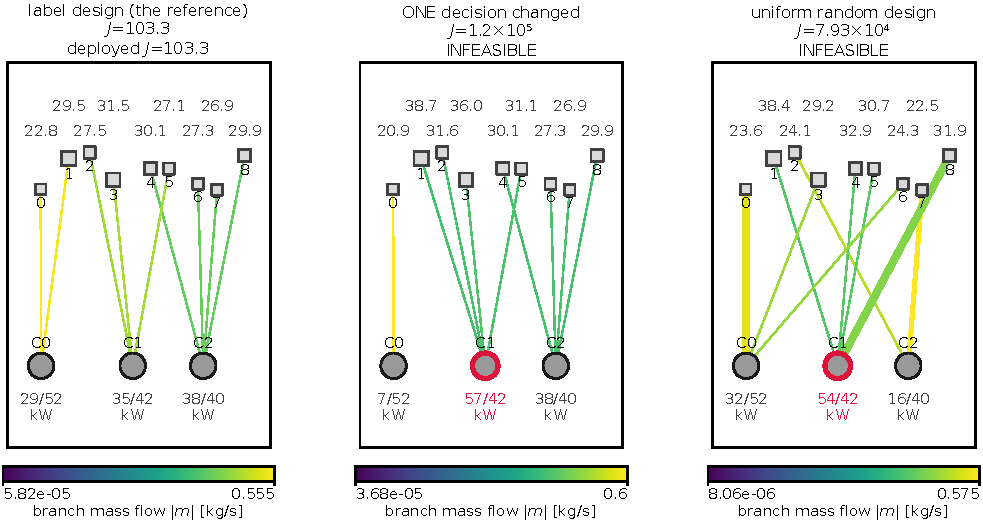
\includegraphics[width=\linewidth]{figures/fig_lc_layout.pdf}
\caption{A Benchmark-B design on the physical layout: racks (squares) and CDUs
(circles, duty against rating) at their true coordinates.  Pipes are
coloured by solved branch mass flow and widened by diameter class, and a red
outline marks a violated limit.  The two rows of numbers above each panel are the solved rack-outlet
and CDU-supply temperatures in $^\circ$C.  \emph{Left:} the feasible label design, $J=103.3$.  \emph{Middle:}
one assignment decision changed, infeasible at $J=1.2\times10^{5}$.  \emph{Right:} a
uniform random design, infeasible at $J=7.9\times10^{4}$.  Flows, temperatures,
pressures and duties are the solver's; junction nodes carry no positions, so runs are
straight.
}
\label{fig:lclayout}
% source: ddl/case/benchB/E0c_field_snapshots/loggers/20260915T100812Z_gpuserver/
%         results_field_snapshots.json -> tasks[seed=900048].designs.
\end{figure*}

One asymmetry between the benchmarks governs how every
Benchmark-B objective value may be read: the temperature-violation term is
unclamped, unlike the repaired synthetic benchmark's $100$\,K cap.  On grossly
infeasible decodes the realised violation therefore reaches $1.1\times10^{5}$, and
the deployed objective is a hinge magnitude rather than a physical cost.  Feasibility and every
physical quantity in this paper come from the solver's own constraint flags, not from
the objective.

Benchmark~A is ours, which is reason enough to distrust it: the relaxation maps and
the solver were designed together.  \subsection{Benchmark B: the liquid-cooling network of \platform}
\label{sec:benchB}
Benchmark~B therefore keeps the same decision
structure and replaces the physics with the liquid-cooling backend of \platform
~\cite{li2026dctwin}, which was written for facility simulation and not for
this paper.  Its hydraulics are Darcy--Weisbach with a Swamee--Jain friction factor blended
across the laminar transition.  Its pumps follow affinity-law curves, and its CDUs
are NTU-effectiveness heat exchangers.  The steady state is found by the Global Gradient
Method~\cite{todini1988gga}.  A task is $N$ racks with cold plates and $K$ CDU loops, each anchored by an
expansion tank.  The pipe catalogue is the same $M{=}3$ classes.  Positions are
sampled so branch lengths are metres to tens of metres.

Three things had to be built before the backend could be used as a differentiable
reward, and they are worth stating because they are what a practitioner adopting this
recipe will also face.  First, the package exposes no adjoint, so we attach one.  The Newton iteration is
run to convergence without gradient tracking, and the implicit function theorem is
applied at the converged point.  The iteration's data-dependent trip count, its
clamped Jacobian and its internally detached derivatives therefore never enter the
gradient path.  The saddle-point system is
reduced by the same Schur complement $S=A\,G^{-1}A^{\!\top}$ that the solver already
assembles, and $S$ is symmetric.  The adjoint therefore costs one further dense
solve on the reassembled Schur complement; at these problem sizes
($n_{\mathrm{free}}\approx19$--$25$) the forward factorisation is not retained.  Second, the graph compiler converts every physical quantity to a floating-point
scalar, so no gradient can reach a design parameter.  We compile once for structure
and then substitute differentiable parameter tensors.  The head-loss routines
consume those tensors unchanged.  Third, the production thermal march runs under \texttt{no\_grad} with scalar Python
loops.  The flows are frozen once the hydraulics are solved, so we instead assemble
the steady-state node temperatures as a linear system and solve it directly.
Upwinding is smoothed so that the small parasitic flow in a nominally closed branch
has a well-defined direction.
% source: ddl/case/benchB/E0c_field_snapshots/loggers/20260915T100812Z_gpuserver/
%         results_field_snapshots.json -> tasks[seed=900048].designs (Fig. 2 panel
%         titles, the 1.1e5 realised violation, the three deployed objectives).

The hydraulic Global Gradient path and its sparsity pattern are untouched.  The
thermal march is replaced by a linear steady-state solve with smoothed upwinding,
so the exactness claim covers the hydraulics and the substituted thermal block.



\subsection{Benchmark A: enumerable differentiable thermo-hydraulic network}
\label{sec:benchA}
Each task has $N$ racks with heat loads $q_i\in[10,40]$\,kW, $K$ coolant
distribution units (CDUs) with quadratic pump curves, and a catalogue of $M=3$
pipe classes.  A design assigns every rack to one CDU and one pipe class ($2N$
typed decisions, $(KM)^N$ designs).  Steady-state flows follow a regularised
quadratic pipe law with nodal mass balance, solved by damped Newton; outlet
temperatures follow from energy balance.  The objective is pump power$/100$ +
$0.05\times$pipe cost + hinge penalties ($\lambda(v+v^2)$) on rack outlet
temperature ($T_{\lim}=45$\,$^\circ$C) and CDU capacity.  A forward+adjoint
evaluation costs 7\,ms on CPU, so ground truth is available by enumeration for
$N\le4$.  For larger $N$ the reference $\Jobj^\star$ is \texttt{best\_known()}:
the minimum over a full-neighbourhood steepest descent, a coordinate sweep and a
refine from five shared starts, exhaustive whenever $(KM)^N\le8000$.  On the $12$
of $40$ evaluation rows small enough to enumerate, the reference equals the true
optimum exactly, median, mean, maximum and minimum alike.  Regret on the
remaining $28$ rows is therefore an upper bound.  The reference is also \emph{beaten} on $9$ of $40$ rows by the converged search.  On
the $28$ non-enumerable rows regret is therefore a signed gap to a heuristic
reference; $21$ of $292$ archived rows are negative.
% source: ddl/case/policy/inference_search/loggers/20260914T184924Z_gpuserver/
%         results_inference_search.json -> rows with negative regret (9 of 40 for
%         steepest_full; 21 of 292 across arms).
Minimising $\Jobj$ under a saturated temperature penalty does not imply feasibility: the true optimum is
feasible on $6$ of $16$ validation and $6$ of $16$ test rows only.
% source: ddl/case/policy/greedy_and_oracle/loggers/20260915T092629Z_gpuserver/
%         results_greedy_oracle.json -> reference_slack (12 rows scored, slack 0.0,
%         nonneg frac 1.0); enumeration counts archived with the run.

\subsection{Relaxation maps for Benchmark B}
Benchmark B regularises in mass flow, not in pressure: $|\dot m|=\sqrt{\dot
m^2+\varepsilon^2}$ at $\varepsilon=10^{-8}$\,kg/s, which is $C^\infty$ in $\dot
m$, so the smoothness caveat of Benchmark A does not apply here.  At the audited
vertex designs the smallest $|\Delta p|$ over all edges is $1.16$--$3.18$\,kPa and
the smallest $|\dot m|$ is $2.0\times10^{-5}$--$4.4\times10^{-5}$\,kg/s, below the
thermal floor of $10^{-4}$\,kg/s. That is exactly the inflation disclosed in
\cref{sec:e0lc}.  Benchmark B's pump law carries no check valve; every archived
state has positive pump flow (minimum $0.0216$\,kg/s), so that guard is empirical
rather than structural.  The forward solve clamps the friction Jacobian at
$10^{-4}$\,Pa\,s/kg while the adjoint clamps at $10^{-8}$. The smallest $|g|$
observed at the audited designs is $1.4\times10^{4}$, eight orders above the forward clamp and twelve above the adjoint clamp, so the mismatch is inert.
% source: ddl/case/benchB/E0g_vertex_adjoint/loggers/20260915T225434Z_gpuserver/
%         results_vertex_adjoint.json -> min_abs_dp_Pa, min_abs_m_kgs; pump-flow
%         minimum from ddl/case/benchB/E0c_field_snapshots/loggers/
%         20260915T100812Z_gpuserver/results_field_snapshots.json.
The assignment relaxation exploits an algebraic accident of the Darcy--Weisbach
form.  A pipe's resistance coefficient is $(fL/D+K_{\mathrm{minor}})/(2\rho A^2)$,
and the friction factor $f$ depends only on the Reynolds number, hence not on $L$
or $K_{\mathrm{minor}}$.  Dividing both
by a weight $w$ therefore multiplies the coefficient by exactly $1/w$.  The
network carries every candidate branch as a real pipe edge, and a soft assignment
sets $w_{ik}=C_{\min}+z_{ik}(1-C_{\min})$ in the solver's own friction law.  A
one-hot $z$ compiles to the hard design up to the conductance floor $C_{\min}$ of Supplementary Table~S-VI, and every
probability vector yields a network whose node
degrees, sparsity pattern and Newton iteration are identical.  The $1/w$ scaling
is exact because every node shares one elevation; a gravity head would break it,
the first assumption to revisit in a real-facility extension.  For the catalogue
we compare the expected diameter $\sum_j p_jD_j$ against the diameter carrying
the expected $1/D^5$ resistance, $(\sum_j p_jD_j^{-5})^{-1/5}$.

\subsection{Relaxation maps for Benchmark A}
The regularised pipe law of Benchmark A is $C^1$ at $\Delta p=0$ with
$f'(0)=1/\sqrt{\varepsilon}$ at $\varepsilon=10^{-3}$\,kPa, but not $C^2$.  Newton
is therefore only linearly convergent on branches whose $\Delta p$ crosses zero,
and a central difference across such a direction is $O(h)$.
% source: ddl/src/thnet.py EPS_DP and the six-task |dp| audit recorded in
%         ddl/docs/FINDINGS_2026-09-15.md s51.
CDU assignment: row-softmax $z_i\in\Delta^K$ mixes conductances linearly,
$C_{ik}=C_{\min}+z_{ik}(C^{\max}_{ik}-C_{\min})$ with $C_{\min}>0$ (physical
closure).  Pipe class: $b_i\in\Delta^M$ gives an expected $D^5$ (``D5'') or an
expected resistance (``harmonic'').  A geometric (log-conductance) interpolation
is included as a negative control.

\subsection{Policies and estimators}
For estimator analysis we use a factorised categorical policy (one softmax per
decision) so that the exact gradient of $\E[\Jobj]$ can be computed by
enumeration ($N{=}4$) or estimated with 2048 score-function samples.  For post-training we use Qwen3.5-4B with LoRA rank 16 on all projections
($2.38\times10^{7}$ trainable parameters, one 96\,GB GPU).  No 27B run is reported here (\cref{sec:e27b}).  Both decode under
grammar constraints over the \ddl{} scaffold.  The base model with adapters disabled
serves as the KL reference.  Designs are sampled autoregressively at decoding temperature $1.0$ in every
run reported here; that temperature, not $\tau$, sets the spread of the $G$
designs whose objectives the estimators average.  Estimators: REINFORCE with
leave-one-out baseline, GRPO (group-normalised advantage), pathwise
straight-through (conditional Gumbel, backward temperature $\tau$), pathwise soft
(no straight-through), and a fixed-weight mixture.  Physics runs on a second
GPU; only the soft design and its adjoint cross the device boundary.

\FloatBarrier
\section{Results}
\label{sec:experiments}

Every number in this section names its benchmark, its seed count and its physics
configuration, and is traceable to a JSON artefact in the companion repository, as
the Code and Data Availability statement describes.  The synthetic benchmark is the
repaired revision: its pump model carries a check valve and the rack outlet
temperature cap is $100$\,K.  The physicality audit that motivated the repair,
and its enumeration verification, are Supplementary Sec.~S-X.  The earlier revision, which carried neither, admitted non-physical designs
(reverse pump flow, $372\times$ capacity overload) and a $1.4\times10^{10}$
objective dynamic range in its enumerated audit.  Under the repaired physics the
same audit gives a $4.05\times10^{4}$ dynamic range and six non-physical designs.  Every estimator and post-training result
in this section is measured under the repaired physics.  Post-training on the
synthetic benchmark is reported at five seeds per arm (\cref{sec:e2}); on the
production solver each arm is reported at the seed count \cref{sec:e2B} states.
The subsections report their verdicts in order: the adjoint is exact while the relaxation is not
(\cref{sec:e0}, \cref{sec:e0lc}), and fidelity does not predict shipped
quality on the production solver (\cref{sec:e1lc}).  Post-training trades quality
for feasibility on Benchmark~A (\cref{sec:e2}) but regresses against its warm start
on Benchmark~B (\cref{sec:e2B}); scale remains open (\cref{sec:e27b}), and cheap
controls bound what post-training buys (\cref{sec:baselines}).

\emph{Five-seed rule.}  A mean-regret comparison is reported as a result only at
five or more seeds per arm; race-style controls state their task and seed counts
beside every number.  Below five seeds it is reported as a direction, and any
paired test at fewer than six units is quoted together with its exact combinatorial
floor.  No multiplicity correction is applied beyond the two Holm adjustments stated with
their families in Table~I and \cref{sec:e2B}; where a family of tests is printed
together, the caption states how many of them survive.

Before any metric, two figures show what these policies build.  \Cref{fig:fields}
solves three designs of one production task in physical terms: the branch
mass-flow, device-temperature and node-pressure fields on the layout the solver
sees, every panel naming its objective value and its feasibility verdict.
Supplementary Fig.~S11 repeats the comparison over two validation tasks and five
controls, drawing the pipe arrangement each control leaves behind and ringing
every constraint a design violates.  The later figures of this section then
measure what these fields suggest.

\begin{figure*}[!t]\centering
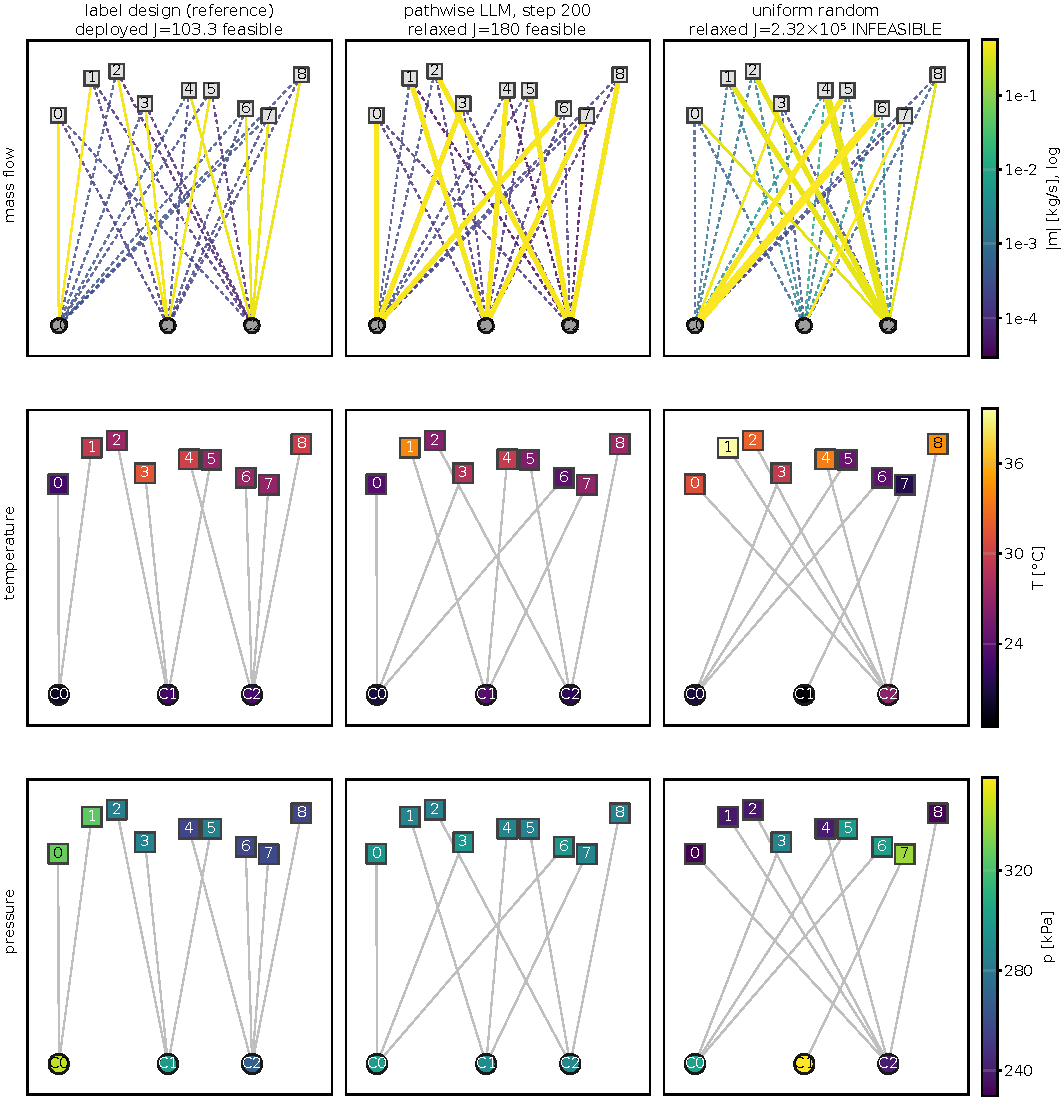
\includegraphics[width=\linewidth]{figures/fig_lc_fields.pdf}
\caption{Solved fields of three designs of Benchmark-B task seed 900048 on the
physical layout: racks 0--8 (squares), CDUs C0--C2 (circles).  Rows are the branch
mass-flow field $|\dot m|$ (log scale, dashed where nominally closed) and the
device temperature field (rack outlet, CDU supply); each row shares one colour
scale.  The node pressure field of the same designs is in the companion repository.
Left, the labelled reference, deployed objective $103.3$, feasible.  Middle, one
pathwise seed (s0) at its final saved checkpoint, shown as an illustration rather
than a measurement, relaxed objective $180$, feasible.  Right, a uniform draw, relaxed objective
$2.32\times10^{5}$, infeasible: rack 1 reaches 39.6\,$^\circ$C against
29.5\,$^\circ$C, CDU C1 is starved to 6.9\,kW and CDU C2 is asked 60.9\,kW against a
40\,kW rating.  Panel titles name each $J$'s functional (deployed re-solve where archived, else relaxed).}
\label{fig:fields}
% source: ddl/case/benchB/E0d_case_gallery/loggers/20260915T110608Z_gpuserver/
%         results_case_gallery.json -> tasks[seed=900048].designs['llm:final'|'label'|'random']
%         (CDU supply pressures, rack temperatures, CDU duties, panel objectives);
%         middle-panel adapter ddl/case/benchB/E2_llm_posttrain/loggers/
%         v2B_20260915T024854Z/ste_s0/final.
\end{figure*}


The post-trained model balances the three CDU supply pressures to within 10.6\,kPa,
where the reference spreads them over 76.3\,kPa, and holds every rack below its limit at 74\% higher
objective.  The uniform draw starves CDU C1 to 6.9\,kW, overloads C2 to 60.9\,kW against a 40\,kW
rating and runs rack 1 ten kelvin hot; its pressure field is the signature of that starvation.



The estimator comparison is robust to that repair: the matched-budget race and the
bias--variance audit agree with their pre-repair values to three decimals
(Supplementary Sec.~S-I).  All numbers below are from a single workstation with two 96\,GB GPUs; seeds,
configurations and logs are in the accompanying repository.  Benchmark~B (the liquid-cooling network of \platform
network) \emph{is} reported here: \cref{sec:e0lc} covers its adjoint, closure floor
and decision-type split, and \cref{sec:e1lc} the estimator comparison on it. Post-training a language model on that solver is reported at five seeds
(\cref{sec:e2B}); \cref{sec:e2} is Benchmark~A only.

\subsection{The adjoint is exact; the relaxation is not}
\label{sec:e0}

Adjoint gradients agree with central finite differences to a median relative
error of $1.1\times10^{-8}$ (worst $8.5\times10^{-7}$) over 24 checks (6 seeds $\times$ 4 configurations).  Yet the first-order pathwise prediction of a discrete edit's benefit,
$\hat I_1(a)=-\nabla_z\Jobj^\top v_a$, ranks the true re-solved benefits of all single
edits with a mean Spearman correlation of only $0.57$.  Sign accuracy is $77\%$,
top-3 hit rate $63\%$ and top-1 $25\%$.  The objective is monotone along the
relaxation path for only $58\%$ of edits; Supplementary Fig.~S6 draws the ranking.  The relaxation map matters: geometric interpolation collapses the assignment
correlation from $0.54$ to $0.12$, because its slope at a one-hot point is dominated
by $C_{\min}$.
% source: ddl/case/benchA/E0_adjoint_and_edits/loggers/20260914T224553Z_v2/results_e0.json -> aggregate
%         {fd_rel_err_median 1.1326e-08, grad_check[].rel_err_max 8.5196e-07, spearman 0.57167,
%          sign_acc 0.77185, top3 0.625, top1 0.25, path_monotone_frac 0.57523};
%         ddl/case/benchA/E0b_relax_variants/loggers/20260914T224553Z_v2/results_e0_relax.json ->
%         {"z=linear,b=D5".rho_assign 0.54467, "z=geometric,b=D5".rho_assign 0.11726,
%          mono_diam harmonic 0.66406 vs D5 0.61024}.  Round 3 (P0-E) found this paragraph printing the
%         pre-v2 values (1.3e-8 / 0.59 / 78% / 58% / 0.63 / 0.59) under a stamp asserting they were v2.
This is the bias source \cref{sec:estimators} anticipates: local slopes carry
information about discrete edits, but not enough to rank them alone.


\subsection{Does any of this survive a real solver?}
\label{sec:e0lc}
\emph{The adjoint is exact here too.}  Against central differences in the decision
variables, the adjoint we attached to the GGA solve agrees to a median relative error
of $\sim3\times10^{-10}$ (worst $\sim6\times10^{-9}$, 28 directional checks). The check is deterministic: a fresh process reproduces both values
bit-identically, and an earlier differing partner was a different code version,
not a second draw.  The achieved $3\times10^{-10}$ is set by the check's step sizes, not by the
objective scale: an archived sweep from $h=10^{-3}$ to $10^{-9}$ reaches
$6.6\times10^{-11}$ at $h=10^{-5}$ and degrades on either side.  At the one-hot
vertices where the edit-ranking and post-training claims live, the same adjoint
agrees with forward differences to $1.4\times10^{-3}$ at $h=10^{-5}$ and to
$1.4\times10^{-5}$ at $h=10^{-7}$ on closed-branch coordinates. Chosen and catalogue coordinates agree to $10^{-9}$.  A central difference at a
closed-branch coordinate with $h=C_{\min}$ is a $100\%$ relative perturbation of
that branch's weight, so the disagreement of an absolute-step harness there is a
harness artefact, not an adjoint error.
% source: ddl/case/benchB/E0g_vertex_adjoint/loggers/20260915T225434Z_gpuserver/
%         results_vertex_adjoint.json -> per_seed.*.{chosen,unchosen,cat}.
%         {median,max} per h; h-sweep of the interior checks in
%         ddl/docs/FINDINGS_2026-09-15.md s51.  The synthetic solver's checks give $1.1\times10^{-8}$ /
$8.5\times10^{-7}$ over 24 directions and its v2 repair $5.12\times10^{-10}$ /
$2.86\times10^{-7}$ over 288, so this paper quotes orders rather than four
significant figures.

\emph{Physical closure costs little, and the cost is controllable.}
Supplementary Table~S-VI compares a one-hot soft network against the network in which the
unchosen branches are genuinely absent, over 18 random designs.  Physical quantities
are reported rather than $\Jobj$, whose quadratic capacity penalty amplifies a small
physical difference on grossly infeasible designs; $\Jobj$ appears on the feasible
subset only.  At $C_{\min}=10^{-5}$ the relaxed network reproduces pump power to
$0.11\%$, the worst rack outlet temperature to $0.048$\,K and the worst CDU duty to
$1.00\%$ over the feasible designs.  The errors fall as the closure floor is
lowered, except the pump column at the last decade.

Those five numbers are measured \emph{at the reference design}, and
Supplementary Fig.~S8 draws the leakage: every nominally closed branch still carries
a fraction of the open-branch flow at $C_{\min}$.  Sweeping the distance from that
design model-free on validation, the median relative difference holds at
$5$--$6\times10^{-4}$ for $\varepsilon\le0.10$ and then grows by up to two orders of
magnitude, non-monotonically.  On validation $3.8\times10^{-2}$ at $\varepsilon=0.20$
falls to $3.6\times10^{-3}$ at $\varepsilon=0.30$ before rising to $1.3\times10^{-1}$
at $\varepsilon=1.0$.  The test column's median reaches $1.1\times10^{-1}$ at $\varepsilon=1.0$; its worst
case is $2.2\times10^{-1}$ at $\varepsilon=0.20$ and $6.6\times10^{-1}$ at
$\varepsilon=1.0$.  The sweep replaces each decision of the label design with a uniform draw at rate
$\varepsilon$ and scores the relaxed index at the resulting one-hot vertex against
the hard compile.  It covers $317$ scored Benchmark-B designs and $12{,}800$ Benchmark-B
relaxed solves ($25{,}600$ across both benchmarks).
% source: ddl/case/analysis/sampling_tail_control/loggers/20260915T051016Z_gpuserver/
%         results_sampling_tail.json -> results[bench=B].hard_subsample.closure_rel_median
%         and closure_rel_max per eps and split; 317 scored designs, 12,800 Benchmark-B
%         relaxed solves (25,600 across both benchmarks); bracketing points at
%         eps 0.06/0.08/0.10/0.12 from loggers/20260916T011348Z_gpuserver/.
A policy that explores leaves the neighbourhood in which the quoted floor was
measured.  The logged within-batch spread of a post-training run puts it between
$\varepsilon\approx0.00$ and $0.12$ on this axis (three single-seed runs, none with a
done row).  A bracketing sweep at $\varepsilon=0.06/0.08/0.10/0.12$ then measures worst-case leakage
up to $0.369$ on validation and $0.203$ on test within the band.
Benchmark~A gives exactly $0.0$ on all $320$ such pairs, since its relaxed
index at a one-hot design is the deployed objective.  An audit of all $104$ Benchmark-A tasks at one-hot designs finds parasitic
branches carrying up to $44.8\%$ of a rack's inflow and up to $20.2$\,kW on a CDU
the design loads not.  Junction mass balance still holds to
$6\times10^{-12}$\,kg/s: this is closure-floor physics, and the reason closure is
measured on Benchmark~B only.
% source: case/analysis/sampling_tail_control/loggers/20260915T051016Z_gpuserver/
%         results_sampling_tail.json -> results[bench=B].hard_subsample.closure_rel_{median,max};
%         ddl/docs/FINDINGS_2026-09-15.md s30.2; eps calibration of the live runs s30.1,
%         which is a diagnosis from three single-seed runs with no done row.
The leakage column is the mechanism: a nominally closed branch keeps the
conductance floor $C_{\min}$, and therefore keeps flowing; the worst leak falls from
$80.2\%$ at $C_{\min}=10^{-2}$ to $0.23\%$ at $10^{-6}$.  Two qualifications travel with it.  The pressure-reference tanks absorb the
leakage as source and sink ($2.7\times10^{-3}$\,kg/s on the label design,
$0.49\%$ of the largest branch-pipe flow), so a soft design transports a small
mass between hydraulically independent CDU loops.  At the deployed floor the smoothed upwinding weight on
nominally closed branches is $0.51$ (median), so parasitic branches deliver about
half their enthalpy upstream.  The thermal march therefore reads their mass flow
$1.105\times$ (median,
$1.99\times$ worst) above the hydraulic solve.  The thermal energy balance
nonetheless closes to $+3.1$\,W on the label design and $-828$\,W ($-0.81\%$) on a
uniform draw, of $102$\,kW total load.


\emph{The bias transfers, and splitting it by decision type is what the synthetic
benchmark could not show}.  Repeating the edit-ranking experiment of \cref{sec:e0} on
Benchmark~B gives a rank correlation of $0.52$, sign accuracy $0.75$, top-1 $0.42$ and
path monotonicity $0.53$.  Benchmark~A sits in the same regime on correlation and sign
but not on selection: the same harness records Spearman $0.57$, sign agreement $0.77$,
top-$1$ $0.25$ and monotonicity $0.58$ there.
% source: benchA v2 edit ranking, ddl/case/benchA/E0_adjoint_and_edits v2 aggregate ->
%         spearman 0.572, sign 0.772, top1 0.25, mono 0.583 (RESULTS_index row A2).
% source: one run for the whole subsection -- benchB/E0_adjoint/loggers/20260915T001550Z_limitcycle/
%         results_e0_lc.json -> edits_resistance {sp 0.52271, sg 0.75499, top1 0.41667, mono 0.52907,
%         n_skipped_edits 4}.  The older loggers/results_e0_lc.json gives top1 0.50 with 5 skipped edits;
%         round 3 (P1-j) required that a subsection quote ONE run, and this is the run that also supplies
%         the closure table and the limit-cycle counts quoted beside it.
But the aggregate is a mixture of two sharply different behaviours, drawn in
Supplementary Table~S-V.  On
catalogue edits the local slope is almost a perfect predictor (rank correlation
$0.94$, path monotone $78\%$); on assignment edits it is weak (rank correlation
$0.31$, path monotone $28\%$).  The reading is mechanical rather than statistical.  Changing a pipe class perturbs
one branch resistance smoothly.  Moving a rack between CDUs redistributes flow across
shared headers, shifts two CDU duties and can cross a capacity constraint: a large,
strongly non-linear reconfiguration that no local slope should be expected to rank.  Benchmark~A's assignment edits scored $0.54$
against $0.31$ here, so the real network is the harder of the two, which is the
outcome that justifies running it.

\emph{The pathwise estimator's bias is therefore concentrated in the structural
decisions.}  This is a sharper statement than ``the pathwise estimator is biased''.
It suggests a refinement we have not implemented: an estimator mixed \emph{by
decision type}, pathwise for the parametric decisions where it is nearly exact and
score-function for the structural ones.  The equal-weight mixture of the two estimator terms is not reported: it is
dominated by both extremes.

We stress that ranking edits and training a policy are different tasks.  Ranking asks
the gradient to identify the single best modification at one design point; training
asks only that the gradient point in a useful direction on average over many points.
The E2 results are evidence about the second, and are not in tension with the modest
rank correlations here.


Relaxing the production solver admits a non-converging undamped-Newton oscillation
that lives beyond one decision from a good design; the failure counts, rescue
counters and closure-sweep exceptions are Supplementary Sec.~S-XII.

\subsection{On the production solver, fidelity does not predict design quality}
\label{sec:e1lc}
Three arm sets appear here and they are not the same size.  Supplementary
Fig.~S9 records nine arm labels at five seeds, of which eight are distinct on the
deployed objective (the straight-through and all-pathwise arms coincide bitwise
there while differing in fidelity).  The cross-objective correlations cover
fifteen arm-scale pairs at three seeds, and the edit-selection test covers ten
policy points at five seeds.  Each statistic names its own set where it is
quoted.  Arm names: \emph{pathwise} (straight-through), \emph{scalar-reward}
(GRPO), \emph{type-wise control}, three calibrated variants (\emph{global},
\emph{inverse-variance-weighted}, \emph{shrunk}) and two partially calibrated
variants.  The relaxation of a \emph{structural} decision is far less faithful
here: assignment Spearman $0.31$ against catalogue $0.94$, versus $0.54$/$0.53$
on the synthetic benchmark (\cref{sec:e0lc}).  We therefore expected the
pathwise arm to stop paying there and the type-wise arms to take over.  All arms
ran at a matched budget of $400$ physics evaluations, five seeds,
$N\in\{8,16\}$, with solver failures counted rather than dropped.

The opposite happened on the deployed objective, and only there.  At $N=16$ the
global calibrated arm ships the best deployed design ($344\pm39$) and the
pathwise arm ships second ($397\pm224$), $194\times$ better than the type-wise
control arm ($77{,}299$).  On the \emph{relaxed} objective the pathwise arm has
the lowest mean at both scales, but the margins over the guarded calibration
variants sit inside one standard deviation at five seeds.  At \texttt{ddof}=1 the
standard deviations are $0.176$/$0.182$ at $N=8$ and $0.204$/$0.067$ at $N=16$,
so no ordering among the three is resolvable.  What the five-seed race separates
is the surrogate from the shipment: the pathwise arm descends the best relaxed
objective at both scales yet ships third at $N=8$ and second at $N=16$.  The arm-by-criterion matrix is Supplementary Table~S-VII.  No paired test between the pathwise and type-wise arms on the deployed objective
is archived.  At five seeds the exact signed-rank floor $0.0625$ could not reach
$\alpha=0.05$ at any effect size, so none is claimed.
% source: deployed J and the calibrated arms from
%         ddl/case/benchB/E1b_estimator_types/loggers/20260915T150205Z_race5seed_calibbugfix/
%         results_e1b_lc.json (config.seeds = 5) -> race[].greedy[-1][1] averaged over seeds 0-4
%         at N=16: ste 397.5 (sample sd 223.8), calib_global 343.6 (sample sd 39.0),
%         typewise 77299.1, allsf 240836.8.  The 194x is typewise 77299.1 over ste 397.5.
%         summary.race -> N8 ste 0.4172+-0.1578 / calib_global 0.4540+-0.1631,
%         N16 ste 0.6422+-0.1829 / calib_shrunk 0.6645+-0.0600 (sd as archived, n = 5);
%         N16 also gives calib_global 0.8038, typewise_calib 0.8486, typewise 0.8845.
%         Deployed N=8 ordering from the same run: calib_ivw 97.3, typewise_calib 102.2,
%         ste 399.9, allsf 63501.3.  No 13.9x ratio survives anywhere in this paper;
%         the stale 234.28 / 128396.13 / 398321.95 and 0.44169 / 0.43342 / 0.67155 /
%         0.63528 values this comment used to carry came from the three-seed invocations
%         and are not quoted in the body.

\emph{The metric inverts}, as Supplementary Fig.~S9 draws.  Across the eight distinct deployed objectives of the
nine arms the Spearman correlation between fidelity and deployed objective is
$\rho=+0.46$: better-aligned arms ship worse designs.  The tie-aware exact
permutation $p$ is $0.21$, so this is a description of the arm table, not a test.
The scalar-reward arm has the best alignment of any arm ($\cos=0.562$) and a
deployed design of $63{,}501$; the pathwise arm, at $\cos=0.273$, reaches $400$,
$159\times$ better despite aligning half as well.  Against the worst-aligned arm
($\cos=0.075$, deployed $1705$) the same scalar-reward arm is $37.2\times$
worse.  On physical quantities the inversion survives for peak CDU utilisation
($+0.49$), duty margin ($-0.49$), rack outlet temperature ($+0.39$) and deployed
objective ($+0.44$), but dies for feasible rate ($-0.04$) and pump power
($-0.14$).  Alignment predicts neither buildability nor pumping cost.  On
feasible designs zero-physics rules match the exact adjoint: ``move the rack to
the CDU with the most spare rated capacity'' ranks structural edits at $+0.83$
against the adjoint's $+0.10$.  ``Choose the cheapest pipe class'' ranks
catalogue edits at $+0.85$ against $+0.92$, and inverts on infeasible designs
($-0.64$).  The decision-type asymmetry of Supplementary Table~S-V is therefore
attributable in part to that hinge structure and to the ordered-versus-unordered
nature of the two families, not to physics alone.  On the synthetic benchmark the same metric and the same race broadly agree, so
this agreement is itself solver-dependent.
% source: ddl/case/analysis/consistency_inputs/loggers/20260915T154717Z_gpuserver/
%         results_consistency.json -> a_fidelity_vs_deployed["new five-seed invocation"]
%         {rho_deployed +0.46026, n_arms 9, n_distinct_deployed 8, rho_exact_p 0.21455
%         tie-aware, ties_present true, per_arm[].{cos_of_mean_N8, deployed_N8_mean}};
%         allsf cos 0.5618 / deployed 63501.28, ste cos 0.2733 / deployed 399.90,
%         calib_path_only cos 0.0749 / deployed 1705.39, so 159x = 63501.28/399.90 and
%         37.2x = 63501.28/1705.39.  The break-even axes in Sec. VII-H(a) come from the
%         same artefact, block c_breakeven.  Sign convention is the artefact's own:
%         rho_deployed is against J where lower is better, and rho_better_when_lower is
%         the same number negated (-0.46026).  The key this comment used to cite,
%         "spearman_fid_vs_deployed_n8 (-0.1167)", does not exist in this artefact.

\emph{Why a continuous repair cannot work.}  The deployed objective
$\Jobj(\operatorname{argmax})$ is piecewise constant in the logits.  Over $90$
confident-point rows ($15$ arms $\times$ $2$ scales $\times$ $3$ seeds) the
measured descent ratio is exactly $1.0$ in $90$ of $90$, reference gradient
included.  The ratio is $1.0$ in $39$ of $90$ rows at a random point and $0$ of
$90$ at the uniform one.
% source: ddl/case/benchB/E1c_deployed_descent/loggers/20260915T031112Z_gpuserver/
%         results_e1c_deployed_descent.json -> rows[].policy confident (90 of 90
%         ratio 1.0), random (39 of 90), uniform (0 of 90).
A line search on the deployed objective is therefore
not a well-posed estimator comparison at any policy point a trained agent
actually occupies, which is why the protocol below scores \emph{edit selection}
instead.  What the descent test does establish is the decoupling.  Across arms,
fidelity correlates with descent on the \emph{relaxed} objective at
$\rho=-0.468$, where the metric does what it claims against the quantity it is
defined on.  It correlates with descent on the \emph{deployed} objective at
$+0.339$, the wrong sign, and the two objectives' descent qualities correlate at
$+0.075$, essentially zero.  The reference gradient, at $\cos=1.000$ by
construction, achieves a deployed ratio of $0.516$, worse than eight of the
fourteen arms it is used to judge.  These coefficients are computed over $15$
arms, the reference arm included, on one solver at three seeds, excluding the confident rows where a third of
the data ties. Including them moves all three without changing a sign, and none
reaches $\alpha=0.05$ at $n=15$, so they are corroboration, not evidence.
% source: the three coefficients from
%         ddl/case/benchB/E1c_deployed_descent/loggers/20260914T223127Z_postbugfix/
%         results_e1c_deployed_descent.json -> correlations (15 arms, uniform + random policy points);
%         the confident-point degeneracy and the 0/39/90 gradient from
%         loggers/20260915T031112Z_gpuserver/results_e1c_deployed_descent.json -> rows[].policy ==
%         "confident", built identically to case/benchB/E1e_calibration_slopes' confident point
%         (8x one_hot(argmax(randn))).  Round 3 (P1-b) found this comment naming the pre-fix 13-arm run
%         20260914T204016Z_gpuserver, whose coefficients row B9 says must not be quoted.

\emph{Edit selection is the well-posed replacement, and it is measurable.}  At a
hard design every single-decision edit can be enumerated and simulated exactly,
and each estimator's first-order prediction ranked against the truth.  The
harness is validated by a deterministic probe: the exact adjoint at the one-hot
design, with no sampling, must reproduce the independently measured split of
\cref{sec:e0lc}.  It does on the catalogue side ($0.918$ against $0.94$) while
understating the structural side ($0.104$ against $0.31$).  Catalogue $\rho=0.918$ and structural
$\rho=0.104$ with top-1 hit $0.80$ over ten measurements, against $0.94$/$0.31$
from the direct measurement.  Against that reference every stochastic estimator
loses ground.  The best, the type-wise control arm, matches on correlation
($0.511$ versus $0.532$) at $36\times$ lower mean cost when wrong (miss cost
$15.8$ versus $572$; three seeds, $n=6$; the five-seed correlations are $0.435$
versus $0.477$).  That ratio reflects a single catastrophic miss among six
measurements, not typical behaviour.  At five seeds the scalar-reward arm is uncorrelated with the
truth at a confident policy point ($+0.0001$), and per-block affine calibration
is anti-correlated there ($-0.113$).  Supplementary Fig.~S10 splits the same
harness by decision type at a confident policy point, where the exact adjoint
reaches $\rho=0.918$ on catalogue edits against $0.104$ on structural ones.
Paired over those ten confident policy points (five seeds $\times$ two scales),
the exact adjoint out-ranks the scalar-reward arm on every statistic: Spearman
$0.477$ against $+0.0001$, and top-1 edit hit $0.80$ against $0.20$.  An exact
signed-rank test on the per-point Spearman differences gives $p=0.00195$ one-sided
($0.0039$ two-sided).
% source: ddl/case/benchB/E1d_edit_ranking/loggers/20260915T150207Z_edit5seed/
%         results_e1d_edit_ranking.json -> rows[policy=confident]; paired exact
%         signed-rank computed 2026-09-16 over the ten (seed, scale) points,
%         recorded in ddl/docs/FINDINGS_2026-09-15.md s50.
% source: five-seed edit selection from
%         ddl/case/benchB/E1d_edit_ranking/loggers/20260915T150207Z_edit5seed/
%         results_e1d_edit_ranking.json (config.seeds = 5, points random+confident,
%         N in {8,16}, n = 10 policy points) -> summary["confident|exact_adjoint"]
%         {spearman 0.4769, spearman_diam 0.9179, spearman_assign 0.1040, top1_hit 0.80,
%         top1_hit_diam 0.80}, summary["confident|allsf"].spearman +0.00014 (the
%         scalar-reward arm), summary["confident|calib_path_only"].spearman -0.11262,
%         summary["confident|ste"] 0.3776, ["confident|reinforce"] 0.1564,
%         ["confident|grpo"] 0.0954, ["confident|reference"] 0.2585.
%         The n=6 disclosures in this paragraph (0.511 against 0.532, 36x, miss cost
%         15.8 against 572, Spearman span 0.143-0.740, top-1 5/6 and 0.833/0.333,
%         3,432.63) are from the THREE-seed run
%         ddl/case/benchB/E1d_edit_ranking/loggers/20260914T211735Z_gpuserver
%         -> summary["confident|typewise"] 0.5110 and ["confident|exact_adjoint"] 0.5317,
%         and are labelled n=6 (2 scales x 3 seeds) in the text.  They are the only
%         values in this paragraph not reproduced at five seeds; carrying them over is
%         outstanding.  Independent decision-type split 0.94 / 0.30:
%         ddl/case/benchB/E0b_split_decision_type/loggers/20260916T012509Z_gpuserver/
%         results_e0_lc_split.json -> resistance.diam.sp 0.9398 and
%         resistance.assign.sp 0.3069 (6 seeds x 2 reps = 12 designs per variant,
%         1 non-convergent cell skipped in the linear variant; config and per-seed
%         counts in the same file).

Per-block affine calibration reverses the catalogue ranking and is undefined at a
confident policy point; the 24-refit slope census and the two guarded variants are in
Supplementary Sec.~S-I.

\emph{No arm wins every criterion}, and the paper should not imply one does.  On
the relaxed objective at $N=16$ the five-seed point estimates order pathwise
($0.642$) $<$ shrunk ($0.665$) $<$ global ($0.804$) $<$ type-wise calibrated
($0.849$) $<$ type-wise control ($0.884$).  With standard deviations of
$0.067$--$0.267$ the first two are not resolvable.  On the deployed design at
$N=8$ the ordering begins inverse-variance-weighted ($97$) $<$ type-wise
calibrated ($102$) $<$ pathwise ($400$), while the scalar-reward arm ships
$63{,}501$.  That the exact adjoint edits well while its stochastic estimates edit poorly
is the point of the section.  One three-seed instability constrains
practice: the soft forward variant delivered the best deployed design at $N=8$
($95$, three seeds) but diverged at $N=16$ to $9.386\pm4.972$ times its starting objective.
The straight-through variant with a hard forward pass is stable at both scales.

Every estimator comparison should report $\|\hat g\|$ alongside its accuracy
statistics: an arm whose norm is orders of magnitude below its neighbours' has not been measured badly; it has not been measured at all. (The calibrated arms
initially returned norms of $5.8\times10^{-13}$ against $5.4\times10^{7}$ for the
pathwise arm they were derived from, invisible to a race that unit-normalises
every step).  The bias--variance audit of these
estimators is Supplementary Sec.~S-I. At $16$ decisions every estimator is poor
(cosine $0.34$ score-function against $0.59$ pathwise), and as decisions grow the
score-function family degrades to $0.25$ while the pathwise family holds $0.57$
at $2$--$3\times$ higher signal-to-noise.

\subsection{Post-training a language model}
\label{sec:e2}
\cref{tab:e2} reports, and Supplementary Fig.~S7 draws the regret curves. Together they report Qwen3.5-4B with LoRA (rank 16,
$2.38\times10^{7}$ trainable parameters) after a 120-step supervised warm start
on 64 training tasks, then 200 post-training steps at five seeds per arm under
Benchmark~A v2 physics.  The reported score-function configuration is one of
three shortlisted from an eighteen-configuration screen.  The shortlist retains
configurations that never beat the warm start, and at step 200 all three are
worse than it on validation mean-of-medians ($4.96\times$ / $9.55\times$ /
$8.95\times$).  The arms are matched on post-training steps,
not on solver invocations.
% source: step-200 eval.val.agg.regret_median, mean over five seeds, in
%         ddl/case/llm/V2_4b_estimators/loggers/{grpo_lr2e-5_clip3s_G16,
%         grpo_lr2e-5_rank_G8, grpo_lr5e-5_clip3s_G8}_s0..s4/log.jsonl
%         (5.3759 / 10.3524 / 9.6995); ratios against the warm start's step-0
%         value 1.0842 of the same key.
% source: ddl/case/llm/V2_4b_estimators run configs and stdout wall clocks,
%         aggregated in ddl/docs/RESULTS_index.md rows L3-L6 (A: 3,200 fwd + 3,200
%         adj vs 6,400 fwd, 4,359 s vs 13,133 s; B: 12,800 vs 3,200, 11,689-
%         14,901 s).
On Benchmark A the pathwise and type-wise arms pay
$3{,}200$ forward and $3{,}200$ adjoint solves against the score-function arm's
$6{,}400$ forward, at $4{,}359$\,s against $13{,}133$\,s wall clock. On
Benchmark B the ordering inverts ($12{,}800$ invocations against $3{,}200$, at
$11{,}689$--$14{,}901$\,s).  No comparison in this paper is wall-clock matched.
The global gradient clip attenuates every loss term by $\min(1,1/\|g\|)$. On Benchmark A the median clip factor is $7.9\times10^{-3}$ in the pathwise arm
against $3.7\times10^{-1}$ in the score-function arm, so the KL and replay
anchors act about $47\times$ weaker where the physics gradient is large.  On
Benchmark B the factors are $0.69$/$0.81$/$0.77$.  This is a live confound of any
feasibility gain in the pathwise arm and this paper does not resolve it.

On the primary statistic (mean of per-seed true medians) the pathwise arm sits at
$0.571\pm0.073$ / $0.320\pm0.089$ / $0.267\pm0.035$ against the warm start's
$1.084$ / $4.157$ / $7.474$.  Pathwise post-training improves on the warm start in
mean regret on every split. The primary test---one pair per task on the mean over seeds---separates them
only out of distribution ($p=0.0078$ over eight tasks, the exact floor of that
test).  On validation and test the seed-mean test does not separate
($p=0.71$/$0.12$), because task effects dominate (ICC $0.89$/$0.95$ on validation and test).  The effective $n$ is $17$ of $80$ pooled cells and $9$ of $40$
out of distribution (originally as low as $9$ of $40$ pooled cells).  Pathwise beats
the score-function recipe on all three splits before adjustment
($p=0.011$/$9.2\times10^{-5}$/$0.0078$).  A Holm adjustment over the eighteen
primary tests of \cref{tab:e2} retains two of them: this pair on test and the
score-function-against-type-wise pair on test.  The score-function recipe is
worse than the warm start on validation and test ($p=0.034$/$0.0092$) and
inseparable out of distribution ($p=0.31$); the type-wise control separates from
the warm start on no split.  The pooled per-(seed, task) values are retained in
the table note as a sensitivity analysis, not as the claim.

Feasibility moves with the estimator: $0.525$/$0.637$/$0.750$ for pathwise on
val/test/ood, against $0.375$/$0.375$/$0.000$ for the warm start and
$0.312$/$0.250$/$0.175$ for GRPO.  The design-versus-penalty decomposition
qualifies the improvement.  At step 200 of all five seeds the pathwise arm's objective reduction is
$103.1\%$ penalty. Its design cost rises $10.50\to13.49$ over all sixteen validation
tasks (pipe cost $6.75\to10.41$, pump term $3.75\to3.08$), and $10.57\to13.26$ on the
per-seed subset feasible at both ends (mean $5.0$ tasks).  The archived artefact's
self-cross-check fails only on the three intermediate checkpoints of the SFT
warm-start arm (regret median, worst relative difference $0.727$); every block of
every post-trained arm reproduces its training-time log exactly.  What
post-training buys here is constraint satisfaction.  These are the v2 numbers at five seeds for all
three arms; no 27B run is reported here (\cref{sec:e27b}).
% source: ddl/case/analysis/v2A_table/loggers/20260915T175120Z_gpuserver/
%         results_v2A_table.json (five seeds per arm); screen ranks and clip factors
%         from the same artefact and ddl/case/llm/E2_4b_estimators run configs;
%         decomposition from ddl/case/analysis/J_decomposition/loggers/
%         20260915T225120Z_gpuserver/ verdict.txt tables A1/A3/B (start step 120, end
%         step 200, all five seeds; crosscheck failures confined to sft_s0 ckpt 40/80/120).

\begin{table}[t]\centering\caption{Post-training under the repaired Benchmark~A physics: Qwen3.5-4B, LoRA
rank 16, 200 post-training steps from the shared 120-step warm start, five seeds per
arm.  First line of each row: mean $\pm$ sd over seeds of the seed's true per-task
median regret (sd uses \texttt{ddof}=1).  Second line: mean of the per-task mean
regret, then the feasible rate}\label{tab:e2}
\par
% source: every cell of this table and its note, and every paired test quoted with it,
%         from ddl/case/analysis/v2A_table/loggers/20260915T175120Z_gpuserver/
%         results_v2A_table.json -> table.{ste,grpo_lr2e-5_clip3s_G16,typewise},
%         wilcoxon_method exact_dp in every cell.
%         {val,test,ood}.{regret_mean,regret_sd,feas_mean,feas_sd,mean_of_medians},
%         warm_start.{val,test,ood}.{regret_mean,regret_median,feas}, paired_wilcoxon and
%         paired_wilcoxon_seedmean.  That run aggregates
%         ddl/case/llm/V2_4b_estimators/loggers/{ste_s0..s4,
%         grpo_lr2e-5_clip3s_G16_s0..s4, typewise_s0..s4} and ddl/case/llm/V2_sft_4b
%         (warm start) at report_step 200, n_seeds 5, missing [].  The run this comment
%         used to name, 20260915T151413Z_gpuserver, does not exist in the repository.
%         The design-versus-penalty decomposition quoted in the text and in the
%         Conclusion comes from loggers/20260915T225120Z_gpuserver/verdict.txt tables
%         A1/A3/B (start step 120, end step 200, all five seeds, bench A-v2-20260915,
%         checkvalve, dT_cap 100); its crosscheck fails only on sft_s0 ckpt 40/80/120
%         (worst rel diff 0.727 on the regret median).
\footnotesize\setlength{\tabcolsep}{4pt}
\begin{tabular}{@{}lccc@{}}\toprule
arm & val & test & ood\\\midrule
SFT warm start & 1.08 & 4.16 & 7.47\\
 & 10.02 / 0.375 & 12.48 / 0.375 & 13.90 / 0.000\\
GRPO (score-f.) & $5.38\pm4.74$ & $13.44\pm15.69$ & $8.13\pm7.65$\\
 & 21.40 / 0.312 & 35.68 / 0.250 & 25.77 / 0.175\\
pathwise STE & $\mathbf{0.57\pm0.07}$ & $\mathbf{0.32\pm0.09}$ & $\mathbf{0.27\pm0.04}$\\
 & 4.13 / 0.525 & 3.35 / 0.637 & 2.93 / 0.750\\
type-wise & $1.07\pm1.23$ & $0.89\pm0.92$ & $0.48\pm0.28$\\
 & 6.85 / 0.512 & 9.16 / 0.525 & 9.05 / 0.600\\
\bottomrule\end{tabular}
\par\medskip
{\footnotesize First row per arm: mean $\pm$ sd over seeds of the seed's true
per-task median (primary statistic; the warm start is one adapter and carries no
seed spread).  Second row: mean of the per-task mean regret, then the
feasibility rate (its sd over seeds is in the artefact).  Seven of sixteen validation tasks of the warm start carry
regret above $10$ (largest $66.1$), which is why the mean row exceeds the median
row.  The primary paired test is the exact tie-aware signed-rank test on one pair per
task over the seed-mean regret ($n=16$/$16$/$8$); the arm-pair p-triples, the Holm
adjustment and the pooled sensitivity rows are Supplementary Sec.~S-XIII.  The pathwise ood rate is $0.750\pm0.000$ because all
five seeds are feasible on the same six of eight ood tasks.\par}
\end{table}


\subsection{Post-training on the production solver}
\label{sec:e2B}
On Benchmark~B the same recipe trains against the production solver at $48$
training rows against Benchmark A's $64$.  Pathwise and GRPO carry five seeds at
step 200; the type-wise control carries four: its fifth run died at step 178 to a
CUDA device-side assert, is re-running, and nothing here imputes it.  At five seeds
the production solver supplies the paper's sharpest negative: every arm regresses
against its own warm start on regret.  Pathwise is worse on every split in the
pooled per-(seed, task) rows ($p=0.0045$ / $0.00075$ / $0.012$) and inseparable on
the seed-mean primary ($p=0.12$ / $0.18$ / $0.38$).  GRPO is worse on
validation and test on seed-mean ($p=0.034$ / $0.034$), and the type-wise control
diverges ($5.1\times10^{5}$ / $3.2\times10^{5}$ / $879$ against the warm start's
$28$ / $44$ / $69$; seed-mean $p=0.00015$ / $0.0021$ / $0.023$).  Feasibility moves
little and not significantly: pathwise $0.700$ / $0.825$ / $0.650$ against the warm
start's $0.688$ / $0.750$ / $0.625$ (Fisher $p=1$ / $0.49$ / $1$).  A Holm adjustment
over the eighteen seed-mean tests retains five, all of them comparisons against the
diverging type-wise arm.  They are type-wise against the warm start on validation
and test, pathwise against type-wise on validation and test, and GRPO against
type-wise on validation.  Endpoints are not benign either: endpoint-over-best reaches $23$ for
pathwise and $6.4\times10^{5}$ for type-wise (medians $1.47$ / $1.69$ / $37.4$ over
15/15/12 runs).  On the solver where amortisation was supposed to bite,
post-training at 200 steps regresses against imitation training.  The per-split
table, the seed-mean and pooled tests and the feasibility counts are Supplementary
Sec.~S-XI.
% source: ddl/case/analysis/v2B_table/loggers/20260916T033403Z_gpuserver/
%         results_v2B_table.json -> table, paired_wilcoxon (pooled and seed-mean,
%         exact_dp), Fisher counts, endpoint census; type-wise at four seeds with the
%         fifth re-running after a CUDA device-side assert at step 178.
% source: ddl/case/analysis/round10_reanalysis/loggers/20260916T033647Z_gpuserver/
%         results_round10.json -> sec3_holm.benchmark_B.holm_seedmean (5 of 18).


\subsection{The scale question remains open}
\label{sec:e27b}
Every post-training run in this paper is at 4B, so the scale question remains
open and no claim here depends on it.  What the 4B runs establish is that the
mechanism does not require scale at this end: at five seeds one recipe improves
on its warm start out of distribution and the other regresses against it.

\subsection{What a search, a prompt and a 6{,}599-parameter policy achieve}
\label{sec:baselines}

Three controls bound every post-training result, and all three are cheap to run; full per-split numbers are Supplementary
Sec.~S-VI.  Gradient-free full-neighbourhood steepest descent reaches median
regret $0.0673$ at feasibility $0.94$ on validation for a median $186$ physics
evaluations per task.  The arm \texttt{noLLM\_steepest} is capped at $400$ evaluations
with stall limit $3$, and $32$ of $40$ tasks end stalled. Since the oracle that defines regret is itself a
search, no post-training claim here is a single-task-quality claim.  Handing the model the whole simulated single-edit neighbourhood as text improves the
warm start $5.0\times$ on validation; the adjoint's first-order ranking alone, $1.9\times$; both are dominated by the search on every split. A prompt cannot
make the accepted design the one the linearisation ranked.  Two classical designers on the same rows (sensitivity-greedy, alternating
decomposition) beat every learned arm on design quality at $12$ and $514$--$1{,}111$
solves per task, so the claim is amortisation rather than quality (Sec.~S-VI).
% source: ddl/case/policy/greedy_and_oracle/loggers/20260915T092629Z_gpuserver/
%         results_greedy_oracle.json -> sensitivity_greedy, alternating_decomp
%         (same 40 rows, one deterministic pass per task: n_draw_seeds 1).
A 6{,}599-parameter factorised policy post-trained with the same gradient reaches $15.73$ / $9.47$ /
$7.86$ at five seeds, $14.5\times$ worse than the 4B warm start on validation. The mechanism does not require a language model; the one question that does
is Supplementary Sec.~S-III.  A 16{,}260-parameter RackGNN on the same rows reaches $2.25$ / $0.68$ / $1.09$ at five
seeds.  It beats the 4B warm start $6.1\times$ on test, and within one pinned
invocation it beats the factorised policy on all three splits (paired exact
$p=0.0035$ / $8.0\times10^{-5}$ / $0.014$).  Yet it
loses to the post-trained 4B on all three: post-training, not scale or architecture,
is what the language model contributes.  On the factorised policy at a matched
400-evaluation budget the pathwise arm reaches $0.115\pm0.041$ / $0.167\pm0.035$
against REINFORCE's $0.231\pm0.058$ / $0.412\pm0.047$ and GRPO's $0.223\pm0.050$ /
$0.402\pm0.058$ (paired exact $p=6.0\times10^{-8}$ per $N$; Supplementary Sec.~S-I).
% source: ddl/case/benchA/E1d_race/loggers/20260916T011251Z_gpuserver/results_e1d.json
%         -> rows[].{N,task,seed,est,hist}, final/start over the 25 (seed,task) cells per N.
% source: ddl/case/policy/GNN_baseline/loggers/20260915T150746Z_gpuserver_pin1/
%         results_gnn_policy.json -> tests.contrasts[gnn_ste vs mlp_ste].
The fourth control asks whether a learned surrogate removes the case for the adjoint
where solves are cheap.  A per-task MLP trained on $1{,}000$ random hard-compile solves
and descended with its own gradient, at its own cost, reaches $0.206\pm0.137$ (sd, \texttt{ddof}=1) /
$0.229\pm0.105$ against the pathwise arm's $0.124\pm0.043$ / $0.164\pm0.032$ (paired
exact $p=0.012$ / $0.0088$).  It also ships designs an order of magnitude worse in
deployed objective ($1{,}187$ / $3{,}032$ against $112$ / $366$); the matched-budget
variant, the score-function comparison and its held-out error are Supplementary Sec.~S-VI.
% source: ddl/case/analysis/surrogate_baseline/loggers/20260916T021844Z_gpuserver/
%         results_surrogate.json -> rows[].{ste_t0.5,surr400,surr1000,reinforce}.
%         {relax,deployed} and surr_rel_err; paired exact signed-rank over the 25
%         (seed, task) cells per N, method exact_dp.
The endpoint-stability audit of the final checkpoint is Supplementary Sec.~S-VII.
% source: ddl/case/policy/inference_search, ddl/case/llm/E5_prompt_sensitivity,
%         ddl/case/policy/greedy_and_oracle, ddl/case/analysis/run_stability, and
%         ddl/case/policy/small_policy_posttrain/loggers/20260915T150017Z_matched5/
%         results_small_policy.json -> summary["ste|{val,test,ood}"].regret_median_mean.

\section{Discussion and Limitations}
\label{sec:discussion}
\subsection{When the pathwise signal pays, and when it does not}
The experiments delimit a regime rather than assert universal superiority, and
three boundaries are visible.  The advantage grows with the number of decisions.  The matched-budget race of
Supplementary Fig.~S1 and the alignment census of Supplementary Fig.~S5 show the
first boundary: at $N=4$ every estimator is poor, while at $N=16$ the pathwise
direction is twice as well aligned and does not degrade further.  The advantage depends on the relaxation being faithful.  A geometric interpolation
of conductances destroys most of the ranking information the same solver
provides under a linear map; the pathwise estimator inherits that loss and the
score-function estimator is indifferent.  Combining the two signals is not
automatic: the equal-weight mixture is not reported, and a
control-variate coefficient fitted online is the most concrete piece of
unfinished method work here.

\subsection{Limitations}
\emph{Single-step design.}  The agent emits one complete design per episode and
is scored on it; a closed revise loop is not modelled.

\emph{What the gradient cannot see.}  The adjoint differentiates the nominal
steady-state objective; contingencies enter only through penalties evaluated at
that point.

\emph{Solver fidelity.}  Benchmark~A is a lumped thermo-hydraulic network:
quadratic pipe resistance, a pump curve and an energy balance per unit, faithful
to the structure of the design problem and coarse in physics.  Whether the same
relaxation maps carry the same information under three-dimensional
conjugate-heat CFD is open.  The mechanism transfers, since Newton-based solvers
expose the same implicit-function adjoint; the bias induced by relaxing a
structural decision may not.

\emph{Cost accounting.}  We report physics evaluations because that quantity
dominates when a simulation takes minutes; at our benchmark's $7$\,ms per solve
the accounting inverts and a smaller designer would likely win.  The regime this
paper targets is the one where the simulator, not the model, is the bottleneck.
A measured scaling of the production solver locates that boundary: one
hard-compile evaluation costs $7$/$13$/$36$/$60$\,ms at $N=10/40/100/200$ racks:
sublinear at small $N$ where a fixed overhead dominates, linear above
$N=40$.  $K$ grows with $N$ as $3/6/10/20$, so the two are not separated.
% source: ddl/case/analysis/solve_scaling/loggers/20260916T1420Z_gpuserver/
%         results_solve_scaling.json (median of three repeats per size).
The accounting therefore makes a falsifiable prediction.  Where one solve takes
minutes, a post-training step is solver-dominated. The pathwise arm's
matched-budget advantage (about a factor two in regret on the factorised policy)
should amortise after $910$ tasks or $13$ solver calls against the
converged-search comparator, or $340$ tasks against coordinate descent.  Where solves take milliseconds the sign flips and
the smaller designer wins; this submission instantiates only the millisecond end.
\emph{Benchmark B is not independent of us.}  Its solver is \platform
of~\cite{li2026dctwin}, maintained in the same repository as these benchmarks, and
the relaxation was inserted into its friction law \ifblindreview during the platform's development~\cite{li2026dctwin}\else by the authors of~\cite{li2026dctwin}\fi.  What
Benchmark B removes is Benchmark A's co-design of physics and relaxation, not
authorship.
% source: ddl/case/analysis/consistency_inputs/loggers/20260915T154717Z_gpuserver/
%         results_consistency.json -> c_breakeven.headline (910.89 tasks, 12.62
%         solves, comparator steepest_full); matched-budget race from
%         ddl/case/benchA/E1d_race/loggers/20260916T011251Z_gpuserver/results_e1d.json
%         (five seeds x five tasks per N; paired exact signed-rank p=5.96e-8 at both N).
Within the network-solver class the minutes regime is therefore unreachable by
scale alone, and every step here is model-bound.  In the minutes regime the
solver share of a step approaches one, which strengthens the variance argument
of the Introduction rather than weakening it.

\emph{Forgetting.}  Our probes (GSM8K with 50 items, an arithmetic probe with 40
items, NLL on held-out generic prompts) are too coarse over this training horizon
to support any claim in either direction. They are reported as instrumentation,
not evidence.

\subsection{Outlook}
Benchmark~B already is the liquid-cooled network of \platform
platform~\cite{li2026dctwin}; the next environment is its air side, where the
same four action types apply to real facility topologies.  Air-side placement
under three-dimensional CFD needs only that the flow solver expose its implicit
adjoint; the open work is the relaxation map for placement.

% ===========================================================================
\FloatBarrier
\section{Conclusion}
\label{sec:conclusion}

We asked whether the Jacobian of a physics simulator, and not merely its output
value, can be routed into the weights of a language-model design agent.  The
obstacle is that a relaxed distribution over design tokens is not, in general,
anything a solver can simulate.  A differentiable design language removes the
obstacle by construction. A typed vocabulary of design actions with a relaxation
map that is consistent (one-hot recovers the hard design) and physically closed
(any probability vector yields a solvable system).  On a production
water-network solver the closure is an identity inside the physics.  Dividing a
pipe's length and minor loss by a weight $w$ scales its resistance by exactly
$1/w$, because the friction factor depends on Reynolds number alone.  Node
degrees, sparsity pattern and Newton path are therefore unchanged.  The
implicit-function-theorem adjoint then reuses the Schur complement the Global
Gradient Method already assembles, matching central differences to a median
relative error of $\sim3\times10^{-10}$, the finite-difference floor; the one-hot
closed-branch exception at $1.4\times10^{-3}$ is in \cref{sec:e0}.

What followed was mostly not what we set out to show: moving a production solver
into a relaxed design space admits roots its original space never reaches.  On
the synthetic benchmark these include reverse pump flow and a $372\times$
capacity overload.  The fidelity
metric this literature reports does not rank arms the way the designs they
produce do: the best-aligned arm ships a deployed design $159\times$ worse than
an arm with half its alignment.  Asked discretely---does the gradient say
which single edit to make---the exact adjoint reaches $\rho=0.477$ and picks the
true best edit in eight of ten measurements. The scalar-reward arm is
uncorrelated at $+0.0001$ and a continuous line search cannot repair the
inversion because the deployed objective is piecewise constant in the logits.
% source: ddl/case/benchB/E1d_edit_ranking/loggers/20260915T150207Z_edit5seed/
%         results_e1d_edit_ranking.json (config.seeds = 5, n = 10 policy points) ->
%         summary["confident|exact_adjoint"] {spearman 0.4769, top1_hit 0.80},
%         summary["confident|allsf"].spearman +0.00014.

The accounting of what post-training buys is not flattering and we report it as
measured.  Over $100\%$ of the pathwise arm's objective reduction is penalty
reduction ($103.1\%$ at step 200, mean over five seeds).  Post-training buys
constraint satisfaction by spending design quality: $10.50\to13.49$ over all
validation tasks, $10.57\to13.26$ on the per-seed subset feasible at both ends.
Per task it loses to two seconds of gradient-free search under the shared
budget.  Handing the simulated neighbourhood as text is not ignored ($5.0\times$ on
validation) yet is dominated on every split, because a prompt cannot make the
accepted design the one the linearisation ranked.  A 6{,}599-parameter factorised
policy post-trained with the same gradient is $14.5\times$ worse than the
language model's warm start in distribution but indistinguishable out of
distribution at five seeds ($p=0.0625$).  The language model's advantage is
therefore concentrated in fitting the training distribution.  The defensible
claims are amortisation and measurement; the open objects are the
minutes-per-solve regime, scale, and a relaxation map for placement under
three-dimensional CFD.
% source: ddl/case/analysis/J_decomposition/loggers/20260915T225120Z_gpuserver/
%         results_jdecomp.json and verdict.txt tables A1/A3/B (end_step 200,
%         n_seeds 5): %penalty 103.1, dcost 10.50 -> 13.49, paired 10.57 -> 13.26;
%         ddl/case/policy/small_policy_posttrain/loggers/20260915T150017Z_matched5/
%         results_small_policy.json (config.seeds = 5) -> 15.73 / 9.47 / 7.86 vs
%         4B warm start 1.08 / 4.16 / 7.47.

\ifblindreview\else
\section*{Acknowledgment}
The authors thank the DCTwin platform team for the liquid-cooling backend and
the reviewers of the conference version for their comments.  Large language
models (GPT-family assistants, OpenAI) were used by the authors for language
editing and for drafting plotting code. Every experiment, number, figure and
scientific claim was produced and verified by the authors, who take full
responsibility for the content.

\fi
\section*{Code and Data Availability}
Benchmarks, training logs and every artefact behind each figure and each table are
generated by the companion repository of this paper.  They will be released publicly
under an open licence at acceptance; until then they are available from the
\ifblindreview authors\else corresponding author\fi\ on reasonable request.

\bibliographystyle{IEEEtran}
\ifblindreview\bibliography{references_blind}\else\bibliography{references}\fi

\FloatBarrier
\ifblindreview\else
\begin{IEEEbiographynophoto}{Tianyu Li}
Tianyu Li is a Ph.D. student at Nanyang Technological University.
\end{IEEEbiographynophoto}
\begin{IEEEbiographynophoto}{Qingang Zhang}
Qingang Zhang is with Nanyang Technological University.
\end{IEEEbiographynophoto}
\begin{IEEEbiographynophoto}{Hoanghuy Nguyen}
Hoanghuy Nguyen is with Nanyang Technological University.
\end{IEEEbiographynophoto}
\begin{IEEEbiographynophoto}{Zhiwei Cao}
Zhiwei Cao is with Nanyang Technological University.
\end{IEEEbiographynophoto}
\begin{IEEEbiographynophoto}{Ruihang Wang}
Ruihang Wang is with Yunnan University, Kunming, China.
\end{IEEEbiographynophoto}
\begin{IEEEbiographynophoto}{Binyang Song}
Binyang Song is with Nanyang Technological University.
\end{IEEEbiographynophoto}
\begin{IEEEbiographynophoto}{Yonggang Wen}
Yonggang Wen is with Nanyang Technological University.
\end{IEEEbiographynophoto}
\fi


\end{document}
